
\documentclass[12pt]{article}
\usepackage{amsmath}
\usepackage{graphicx}
\usepackage{listings}
\usepackage{dsfont}
\usepackage{subcaption}

\allowdisplaybreaks

\usepackage[bottom=2.54cm, top=2.54cm, left=2.54cm, right=2.54cm]{geometry}
\title{Real-time probabelistic forecasts for the 2018 -- 2019 Ebola outbreak in Northern Democratic Republic of Congo}
\author{
  CANDIDATE NUMBER2
}
\date{\today}

\begin{document}
\maketitle


Word count: XXXX

\begin{abstract}
  Abstract

\end{abstract}

\newpage

\tableofcontents

\newpage

\section{Introduction}


Real time modelling of infectious diseases can play a crucial role during disease outbreaks like the ongoing Ebola outbreak in the north eastern Democratic Republic of Congo (DRC). During the previous large outbreak of Ebola in Western Africa in 2014--2015, many different models were developed\cite{chretienMathematicalModelingWest} and used both to increase our understanding of the outbreak and to predict the spread of the outbreak. Estimates were used in official planning\cite{EbolaVirusDisease2014}  and for example to estimate needed bed capacity \cite{camachoTemporalChangesEbola2015}. Disease modelling has also been sucesfully implemented for for example Zika \cite{kobresSystematicReviewEvaluation2019} and influeza \cite{chretienInfluenzaForecastingHuman2014} among many other diseases. To effectively use results from mathematical modelling in an outbreak it is of key importance that modelling outputs are integrated into the outbreak response and decision making \cite{riversUsingOutbreakScience2019a}. This means that forecasts need to be availabel in real-time and be integrated into the outbreak surveillance information flow. In additionmproved communication and embedding of modelling and modellers into the outbreak response is needed. 

For forecasts to be useful in an outbreak situation, the models need to incorporate uncertainty into the predictions\cite{funkAssessingPerformanceRealtime2019, weiCalibrationTestsCount2014,gneitingEditorialProbabilisticForecasting2008}. Without understanding the range of possible outcomes from a model and their associated probabilities it is very difficult to support effective public health action in outbreak situations. Evaluting such probabelstic forecasts requires us to not just assess the accuracy of point predictions, but to assess if the model correctly assess it's own uncertainty. A model that that sucesfully asseses it's own uncertainty is calibrated. We should strive to create well calibrated models that can be updated in real-time and that that are interpretable and can be used in the outbreak response. 

In this thesis, we will describe a framework for flexibly producing probabelistic forecasts and assess how well the resulting models can be used in the onogin Ebola outbreak in north-eastern DRC. We will compare different models to choose the best model and to explore the epidemiology of the current outbreak. 

\subsection{Ebola outbreak in North Kivu and Ituri provinces}
On the 1st of August 2018, the minstry of health in the Democratic Republic notified the WHO about a new Ebola outbreak in the North Kivu province \cite{worldhealthorganizationEbolaOutbreakDRC2018a}. North Kivu is a populous region in north eastern DRC that borders both Rwada and Uganda. By the 27th of September the outbreak had continued spreading and the WHO assessed that the outbreak constiuted a very high national and regional risk\cite{worldhealthorganizationEbolaOutbreakDRC2018b}.

Due to distrust from the local community the outbreak response has been challenging. This has lead to difficulty in tracing contracts, giving vaccinations and treating patients. There have been many episodes of violence directed towards the ebola responders which has led to fatalities and multiple stops in the response work\cite{worldhealthorganizationEbolaOutbreakDRC2018c,worldhealthorganizationEbolaOutbreakDRC2019a}.

During the outbreak, the experimental vaccination rVSV-ZEBOV-GP has been used in a ring vaccination strategy. The vaccine was given under the compasionate use regime and have been evaluated during the outbreak. Preliminary data shows positive signs that this vaccine might provide some protection from Ebola \cite{organizationPreliminaryResultsEfficacy2019}.  been given to health-care workers and children. This outbreak has also seen a randomised trial for medicines to treat ebola. The trial was terminated at the 12th of August due to findings that two of the four drugs that were included showed clear effect of reducing mortaltiy from Ebola, especially with early treatment \cite{nationalinstituteofallergyandinfectiousdiseasesIndependentMonitoringBoard2019}
At the time of writing the outbreak is still ongoing with new cases from 16 health zones and with fears that the disease will spread to larger cities in the area like Goma or accross borders. On the 17th of July the Director General of the WHO decleared the Ebola outbreak a Public Health Emergency of International Concern \cite{worldhealthorganizationEbolaOutbreakDRC2019}. 

\subsection{Modelling of Ebola}

A large number of different mathematical models have been proposed for modelling Ebola, see e.g \cite{chretienMathematicalModelingWest,viboudRAPIDDEbolaForecasting2018}. The models can be divided into categories based on the structure of the models, mechanistic, semi-mechanistic, phenomenological and hybrid models. Mechanistic models are based on a specified mechanism for disease transmission and includes standard compartmental models while phenomenological models do not include any mechanism for disease transmission. An example of a phenomenological model would be an ARIMA model for the incidence. A semi-mechanistic model include some mechanisitc asumptions, but not a full model for disease transmission.

The RAPID Ebola Forcasting challeng in 2018 \cite{viboudRAPIDDEbolaForecasting2018} presented a range of different scenarios of an ebola outbreak that was similar to the west african outbreak and invited different groups to submitt forecasts and compared them. They found that for short-term forecasting was not related to model complexity and that ``light'' non-parametric models were able to do well. The more complex mechanistic models would on the otherhand be better suited to understand the effects of interventions. 

In this thesis we will present a semi-mechanisitc model that includes some mechanisitc assumptions about serial intervals and forces of infection combined with flexible time-series methods. The aim is a flexible model with parameters that are easily interpretable. 

\section{Methods}

\subsection{Data}
We will use daily incidence data from the North Kivu Ebola outbreak as reported by the Ministry of Health in Congo and distributed via the humanitarian data exchange before the 1st of September 2019 \cite{EbolaCasesDeaths}. We will use the incidence of confimed cases at the national and at the health-zone level. We use confirmed cases so that estimates of the reproduction number and other epidemiological parameters correspond only to Ebola and not Ebola and Ebola-like illnesess. Due to the nature of the outbreak and the nature of the data some confirmed cases are later found to not be Ebola. This can lead to days with negative incidence, we have chosen to set any negative incidence to zero. Data are missing for some days, for these days we lineraly interpolate the incidence. 

\subsection{Model}

We consider a model where the daily incidence, $I_t$ follows a modified branching process. Similar models have been considered in \cite{coriNewFrameworkSoftware2013,lloyd-smithSuperspreadingEffectIndividual2005,nouvelletSimpleApproachMeasure2018} and have been used to model Ebola during the 2014-2016 Ebola outbreak in Wester Africa \cite{EbolaVirusDisease2014, internationalebolaresponseteamExposurePatternsDriving2016}. In this class of models each infectious person gives rise to $\nu$ new infections, where $\nu$ is a random variable distributed with an offspring distribution with an expected value given by the reproduction number $R$. We use the serial interval to model the time between each generation of infections. This gives a process where the expected number of new cases at time $t$ is given by the force of infection $\lambda_t$ which is a product of previous incidence weighted by the serial interval $w_\tau$ and the instaneous reproduction number $R_t$. 

\[ E(I_t) = \lambda_t =  R_t \sum^{t-1}_{s=1} I_s w_{t-s}\]

To fully specify the model we need to determine the probability distribution for $I_t$, the serial interval and the reproduction number as a function of time. For the serial interval we will use  a gamma-distribution with mean 15.3 days and standard deviation of 9.3 days as fitted to data from the West-Africa Ebola outbreak \cite{EbolaVirusDisease2014}. Our general approach will be to use a few different spesifications for the $I_t$ probability distribution and for estimating the time-varying reproduction number and then assess which model gives the best fit to the data.

\subsubsection{Offspring distribution}
The offspring distribution gives us the distribution of the number new infections from each infected person. By definition the expected value of this distribution is the reproduction number. The offspring distribution is a discrete probability distribution over the non-negative integers. The simplest such distribution is the poisson distribution, it is given by

\[P(X=k) = \exp{-\lambda}\frac{\lambda^k}{k!}, \]
with mean and variance given by $\lambda$. This distribution implies that the number of new infections over a time interval is described by a constant rate where the chance of a new infection in each small sub-interval is independent.

For a number of diseases it has been shown that the offspring distribution has larger variance than that given by the poisson distribution and has so called superspreaders \cite{lloyd-smithSuperspreadingEffectIndividual2005}. One common way of modelling this over-dispersed distribution is by the negative binomial distribution. The negative binomial distribution describes a process where we have a series of indepdent chances to infect a new interval each with probabilty $p$, where the process continues until we have had $r$ infection chances without an infection. The distribution is given by

\[P(X=k) = {k + r - 1 \choose k} (1-p)^rp^k, \]

with $E(X)=\frac{pr}{1-p}$ and $Var(X) = \frac{pr}{(1-p)^2}$. We will use a parameterisation of the negative binomial distribution where we use the mean, $\mu$ and the dispersion parameter $k$. In this formulation the variance is given by $\mu(1 + \frac{1}{k})$. For $k->\infty$ we get a poisson ditribution. The smaller $k$ is the more the outbreak is dominated by a few super-spreaders and the larger $k$ is the more similar the impact of each infected person is. For SARS it has been found that $k=0.16$\cite{lloyd-smithSuperspreadingEffectIndividual2005}. For the Ebola outbreak in West Africa they found $k=0.53$ using conservative assumptions and data from the network of infections \cite{internationalebolaresponseteamExposurePatternsDriving2016}. The different offspring distributions ca be seen in Figure \ref{fig:offspring}

\begin{figure}[h]
  \centering
  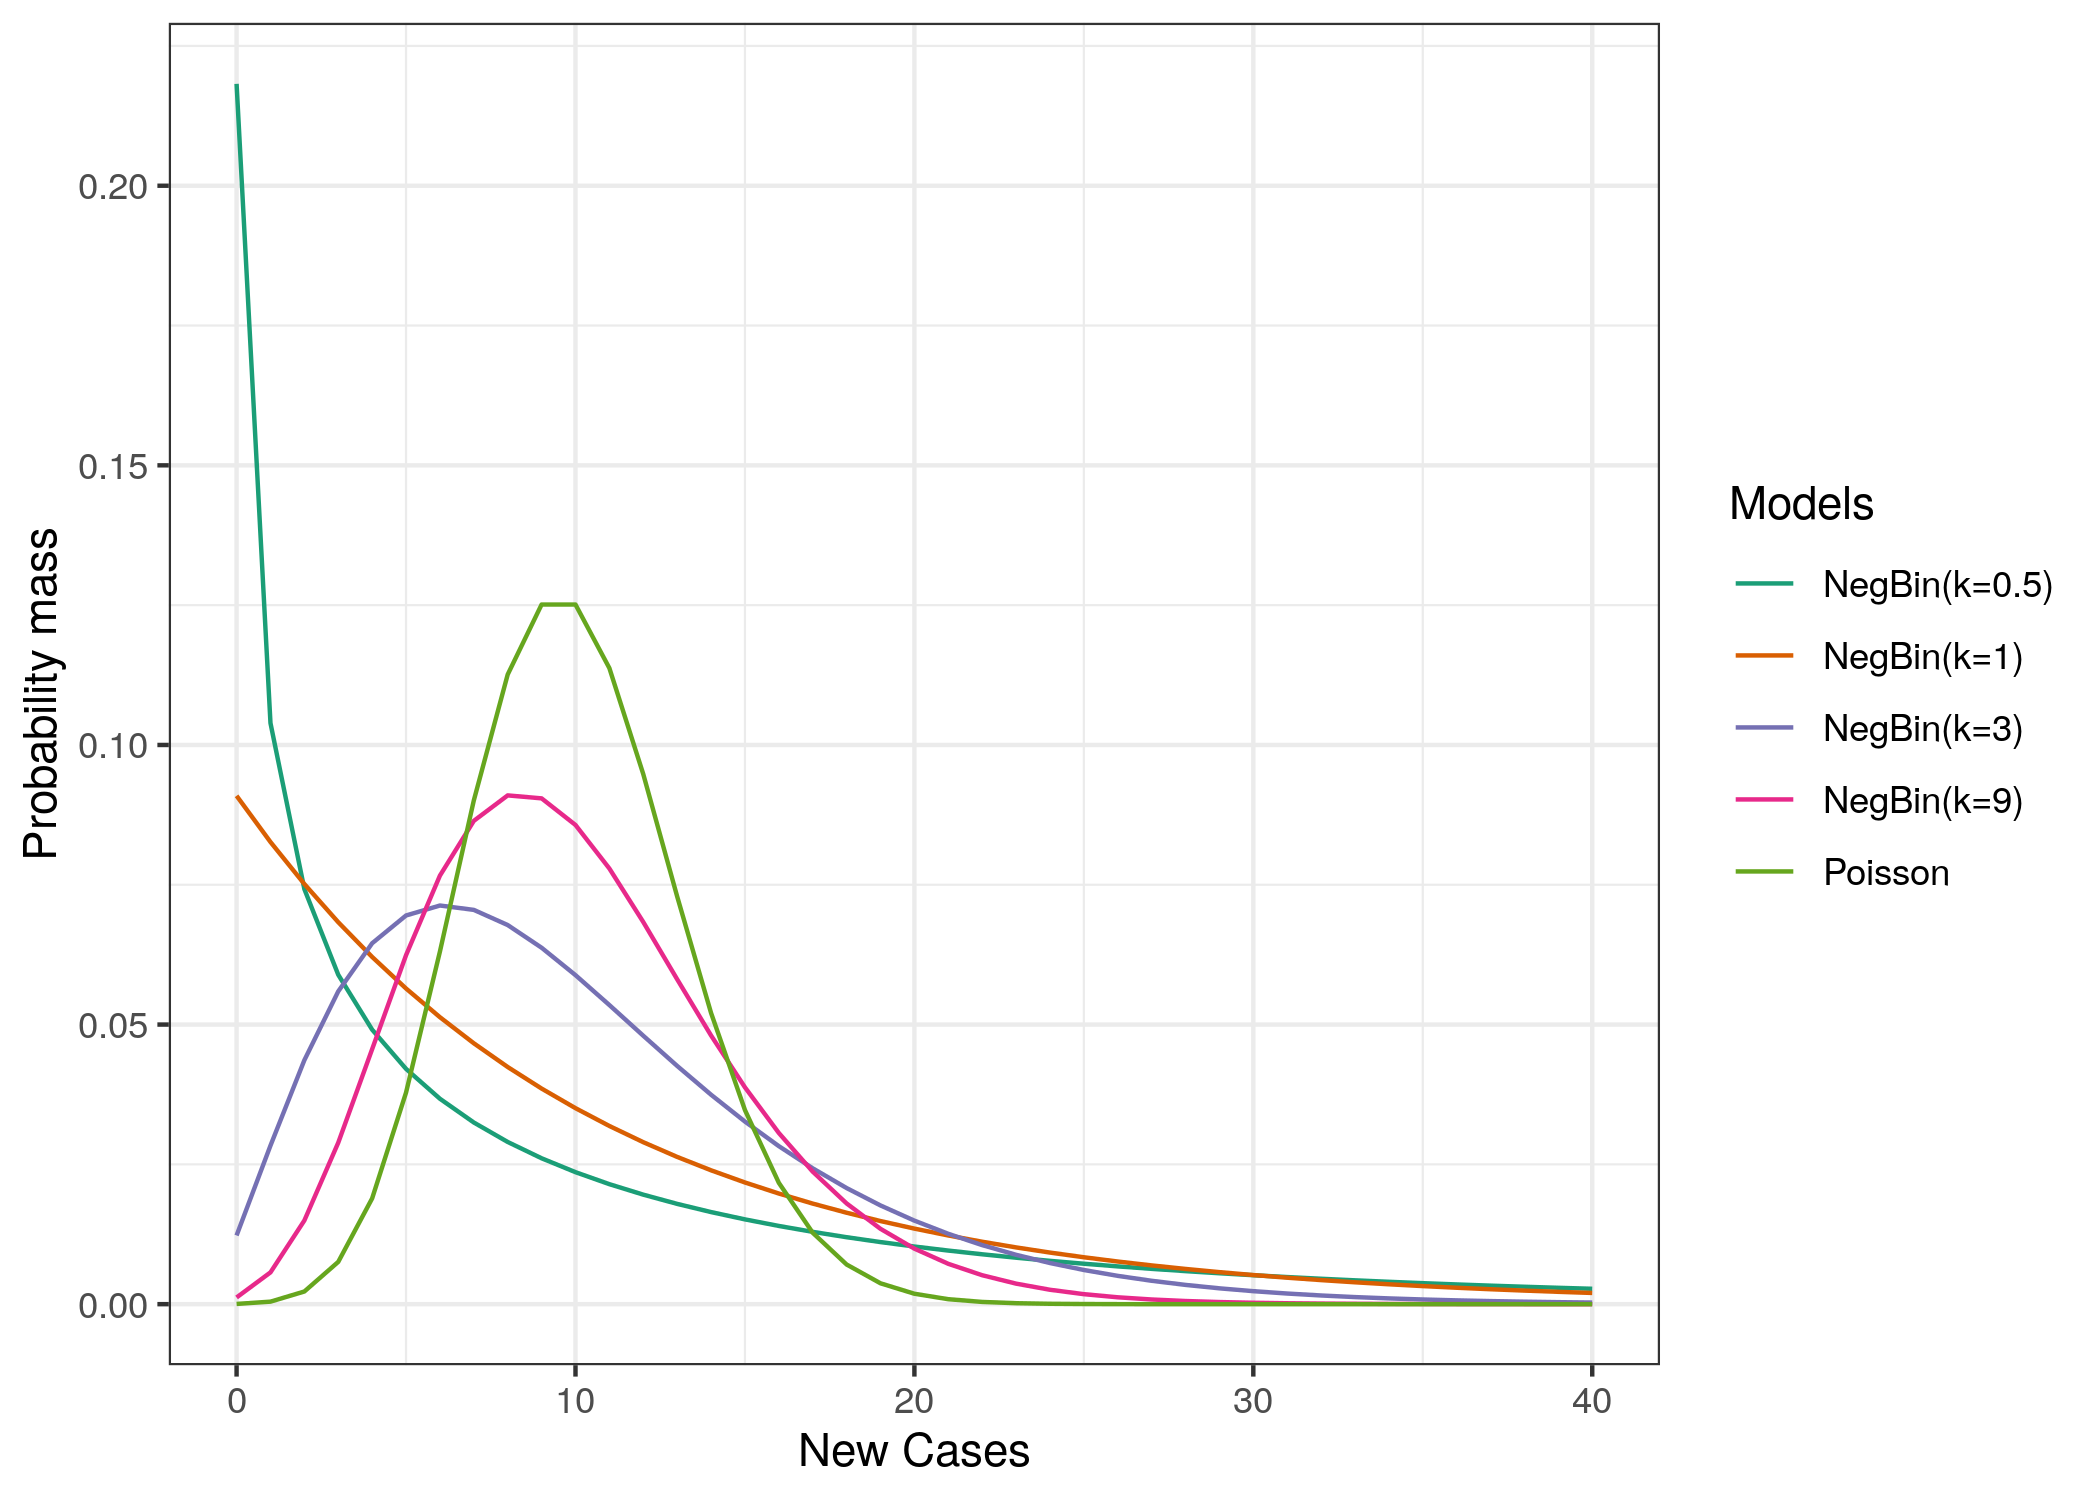
\includegraphics[width=0.7\textwidth]{../output/prob_dist.png}
  \caption{Poisson and negative binomial offspring distirubtions with a mean of 10.}
  \label{fig:offspring}
\end{figure}

The distribution for $I_t$ would be given by the sum of the offspring distributions for each infected person (weighted by the serial distribution). For both the poisson and negative binomial distribution the sum of independent distriubtions will give back the same distribution with an expected value given by the sum of the expected values. For the negative binomial distribution the dispersion parameter $k$ will remain the same. 

We will investigate models with offspring distributions based both on the poisson distribution and the negative binomial distribution to assess which models fit the current outbreak better.

\subsubsection{Reproduction number}
The final ingredient to completely specify the dynamics of the model is the evolution of the reproduction number with time. Depending on the functional form of $R_t$, the model can fit a large range of possible epidemic behaviours. %%The model could for example reproduce in expetation a standard compartmental model where the reproduction number is given by $R(t) = R_os(t)$, where $s(t)$ is the fraction of susceptibles. In a normal SIER model with a constant rate to move between the ``E'' and the ``I'' compartment the serial interval woudl be exponential distributed.

It would be possible to specify a complete model for $R_t$ analytically or otherwise, but in this thesis we will instead estimate $R_t$ from the existing data and use these values to predict the future evolution of $R_t$. Since the focus of the current study is to provide a flexible framework for probabilistic prediction of disease outbreaks, this appraoch is suitable.

To estimate the reproduction number from the historical incidence data we use the method developed in \cite{coriNewFrameworkSoftware2013}. If the reproduction number is estimated daily it is likely to varry too much from day to day in a manner that it is unrelastic. Therefore this method averages over the last 7 days to get more stable estimates. A baysian procedure is used to estimate both the best fit value and the uncertainty of the estimate. We use the R-package EpiEstim \cite{coriEpiEstimEpiEstimPackage2013} to estimate the reproduction number using a parametric gamma distribution for the serial interval with a mean of 15.3 days and a standard devitaion of 9.3 days \cite{EbolaVirusDisease2014}

Once we have calculated the historical values of $R_t$ we can use them to provide an estimate of $R_t$moving forward that can be used for predictions. We will use two different procedures to predict the reproduction number. The first method is a very simple method were we assume that reproduction number remains constant from the last historical value. We use the uncertainties given by the method in \cite{coriNewFrameworkSoftware2013} to provide estimates of the uncertainty of this estimate.

The second approch to predict the reproduction number is based on baysian structural time series fitted to the historical values of $R$. We use model with a semi-local linear trend to allow the estimation of a trend in the recent data. To ensure that predicted values of $R$ are between 0 and 15 we fit the time series on a transfomed scale:

\[ r^* = log\left(\frac{R}{15 - R}\right)\]

We use the R-package BSTS \cite{scottBstsBayesianStructural2019} to fit the basysian structural time series. The model we use is specified as follows

\[r^*_{t+1} = r^*_t + \delta_t + \epsilon_t, \epsilon_t \sim N(0, \sigma_\mu),\]
\[\delta_{t+1} = D + \phi(\delta_t - D) + \eta_t, \eta_t \sim N(0, \sigma_\delta).\]
$\delta_t$ is the semi-local trend that we model as an AR(1) process that can oscilate around a level $D$. Inverse gamma-priors are used for the standar deviation parameters $\sigma_\mu$ and $\sigma_\delta$, a gaussian prior on $D$ and a $N(0, 0.1)$ prior for $\phi$. The $\phi$ parameter determines how much the trend behaves as a random-walk. For $\phi=1$ the trend follows a random walk, while for $\phi=0$ the trend is just constant with some noice. We use a prior for small values of $\phi$ to keep the model for having very rapid growth in the variance of $r^*$ that would be unphysical. 

A Markow Chain Monte Carlo (MCMC) algorithm is used to estimate the parameters in the model which then allows us to predict future values of $r*$ with uncertainties, we then transform back to the $R$. 


\subsubsection{Simulating from the model}
Once we have specified our model by specifying the offspring distribution and the method for forecasting $R_t$ we can use the model to generate probabilistic forecasts. If we want to generate a forecast for $I_{t+1}$ we first use all the data up until time $t$ to estimte $R_t$ and potentially fit the time series model to those values. Our probabelistic forecast will be based on sampling possible outcomes to generate a distribution of outcomes. We therefore first sample a value for $R_{t+1}$ from our model, then we combin this with the historical incidence data to calculate $\lambda_{t+1}$. We then sample $I_t$ from the specified offspring distribution. If we want to forecast over multiple time-steps we follow the same procedure by sampling values for the reproduction number. When calculating $\lambda_{t+2}$ we use the sampled value for $I_{t+1}$ together with the historical data ${I_s}$ for $s\leq t$. 


\subsection{Assessing probabilistic forecasts}
The aim of probabilistic forecasts is to predict both the correct average value and an appropriate uncertainty. Therefore it is not sufficient to only use metrics that depend on a point estimate, for example the Root Mean Square Error. We will follow the paradigm of maximizing sharpness of the predictive distribution subject to calibration \cite{gneitingProbabilisticForecastsCalibration2007}. In addition we will consider proper scoring rules for comparing probability ditributions. We follow the approach taken in \cite{funkAssessingPerformanceRealtime2019}, where probabilistic forecasts for the West African ebola outbreak were assessed using similar methods.

A model is calibrated if the uncertainties are accurate. For example if we predict that it will rain with 60\% and we find that over time it does rain 60\% of days where we predicted a 60\% chance of rain, the model would be well calibrated. Mathematically, if we assume that real disribution of outcomes in nature is given by a cumulative density function $G_t$ and our model predicts a cummulative density function $F_t$, we say that the forecast is ideal and perfectly calibrated if $F_t=G_t$. To assess calibration we will use a randomised Probability Integral Transformation (PIT) \cite{czadoPredictiveModelAssessment2009a}. We calculate
\[ u_t = F_t(k_t) + \nu (F_t(k_t) - F_t(k_t -1)),\]
where $k_t$ is the observed value at time, $t$ and $\nu$ is a standard uniform random variable. If the prediction is ideal, the $u_t$ will be distributed as a standard uniform distribution. We can then use the Anderson-Darling test of uniformity (goftest \cite{farawayGoftestClassicalGoodnessofFit2017}) to assess if we can reject that the models are calibrated. Important to note that uniform PIT is a nescessary, but not suffcient condition for an ideal forecast. In addition to assessing calibration, the PIT histogram can tell us if the forcast is under or overdispersed. If the forcast is too dispersed the PIT values are likely to cluster in the centre of the PIT histogram, while if the forcast is underdispersed they are likely to clusteralong the edges of th histogram. We use a simple measure of centrality, which is equal to the fraction of $u_t$ values that are between 0.25 and 0.75 as a way to assess if the forecasts are under or overdispersed if they are not calibrated.
\[\text{centrality} = \frac{N(0.25 < u_t < 0.75}{N} - 0.5\]
When the centrality scores is less than 0, most of the PIT values or outside of central region suggesting that the forecasts are underestimating the real uncertainty.  If the centrality score is larger than 0 then the PIT scores are mainly in the central region and this indicates that the forecasts are overestimating the amount of uncertainty. 


For both the test for uniformity and centrality we repeat the calculations 10 times and take averages to average out the effect of the randomness in the definition of $u_t$. 

Sharpness is defined as the range of values in the forecast. The sharper a forecast, the more certain we are of predicted value. Sharpness depends only on the forecast and not on the observed values. We will use the normalised absolute devitation about the median of y to quantify sharpness:

\[ S_t(F_t) = \frac{1}{0.675} \text{median}(|y - median(y)),\]
the normalisation factor means that $S_t$ is equal to the standard deviation if $F_t$ is normal.

It is also of importance to assess the bias of the forecast. Are we more likely to predict to large or too smal values? We will qunatify bias as
\[B_t(F_t, k_t) = 1 - (F_t(k_t) - F_t(k_t - 1)).\]
If $B_t=0$ half the probability mass is above and half below the observed value, and the the forecast is unbiassed. $B_t$ is between -1 and 1, with both extreme values signifying a completely biased forecast.

Proper scoring rules have been developed to rank forecasts. They combined calibration and sharpness and give a consistent ranking of forecasts. We will use the the contineously ranked probabilty score(CRPS) and the Dawid-Sebastiani score (DSS) as implemented in the scoringRules package \cite{jordanEvaluatingProbabilisticForecasts2018}. The CRPS score is given by 
\[CRPS(F_t,k_t) = \int_R(F_t(z) - \mathds{1}{k_t \leq z})^2 dz,\]
and the DSS only depens on the mean, $\mu_p$ and standard deviation, $\sigma_p$ of the predictive distribution
\[DSS(F_t, k_t) = \left(\frac{k_t- \mu_p}{\sigma_p}\right)^2 + 2\log\sigma_p.\]
The DSS allows an intuitive understanding of the proper scoring rules. The first term tells us about the calibration of the predictions and the second term gives information about the sharpness. For our models we will only have samples from the predictive distribution. To calculate the CRPS a kernel density estimate is used to estimate $F_t$, for the DSS we use the mean and standard deviation of the sample. 

\subsection{Implementation}
The models were implemented in the R programming langauge \cite{rcoreteamLanguageEnvironmentStatistical2018} and is available open source at http://github.com/gulfa/msc\_ebola. We will consider four differrent models to assess which model fits the data best. The models are:

\begin{enumerate}
\item{Model 1 (Poisson Latest): Constant reproduction number and poisson offspring distribution}
\item{Model 2 (NegBin Latest): Constant reproduction number and negative binomial offspring distribution}
\item{Model 3 (Poisson Semilocal): Varrying eproduction number and poissonoffspring distribution}
\item{Model 4 (NegBin Semilocal): Varrying reproduction number and negative binomial offspring distribution}
\end{enumerate}

For the dispersion parameter $k$ for the negative binomial models we fit a value for the simple negativebinomial model by minimising the continous ranked probability score for the one day ahead predictions for the model on the level of the whole outbreak. 

We will assess how well the models work both for the entire epidemic and for each health zone. To evalute a model we will estimate the calibration, sharpness, bias, log score and CRPS for forecasts of 1, 7, 14, 21 and 28 days ahead. To do this we start { \bf check } 16 days after the start of the epidemic in the location and calculate the $d$ ahead prediction for all historically available data. For the calibration we use all the values to assess if they are normally distributed, while for all the other metrics we average them over all the time steps. 16 days was chosen as the start as this is when the method for calculatng $R_t$ can give somehat reliable values \cite{coriNewFrameworkSoftware2013}. 



\section{Results}
From the start of the outbreak until the 31st of August 2019 there has been 2,926 confirmed ebola cases and 1926 confirmed ebola deaths, this gives a Case Fatality Rate of 66\% compared to 51\% in the west african outbreak\cite{rojekSystematicReviewMetaanalysis2019}. Figure \ref{fig:epi_curve} shows the weekly number of cases and Figure \ref{fig:tot_map} the total number of cases from each Health Zone. From Figure \ref{fig:epi_curve} and the estimte of the instantaneous reproduction number in Figure \ref{fig:rep_num} we can see the evolution of the outbreak. After the initial period were there were no daily surveillance, there was an increase in cases from October 2018 with a large reproduction number, followed by a more varied period where the reproduction number varied around 1 with some waves of larger reproduction number. From March 2019 the number of cases per week increased signficantly, with a continuing large number of cases in June and July even if the reproduction number seems to decrease. From the epi-curve there seems to a connection between the peaks and the large increases in specific health zones. So that pattern is in part driven by introduction or reintroduciton of Ebola to health zones.

\begin{figure}[h]
\begin{subfigure}{0.48\textwidth}
  \centering

  % include first image
  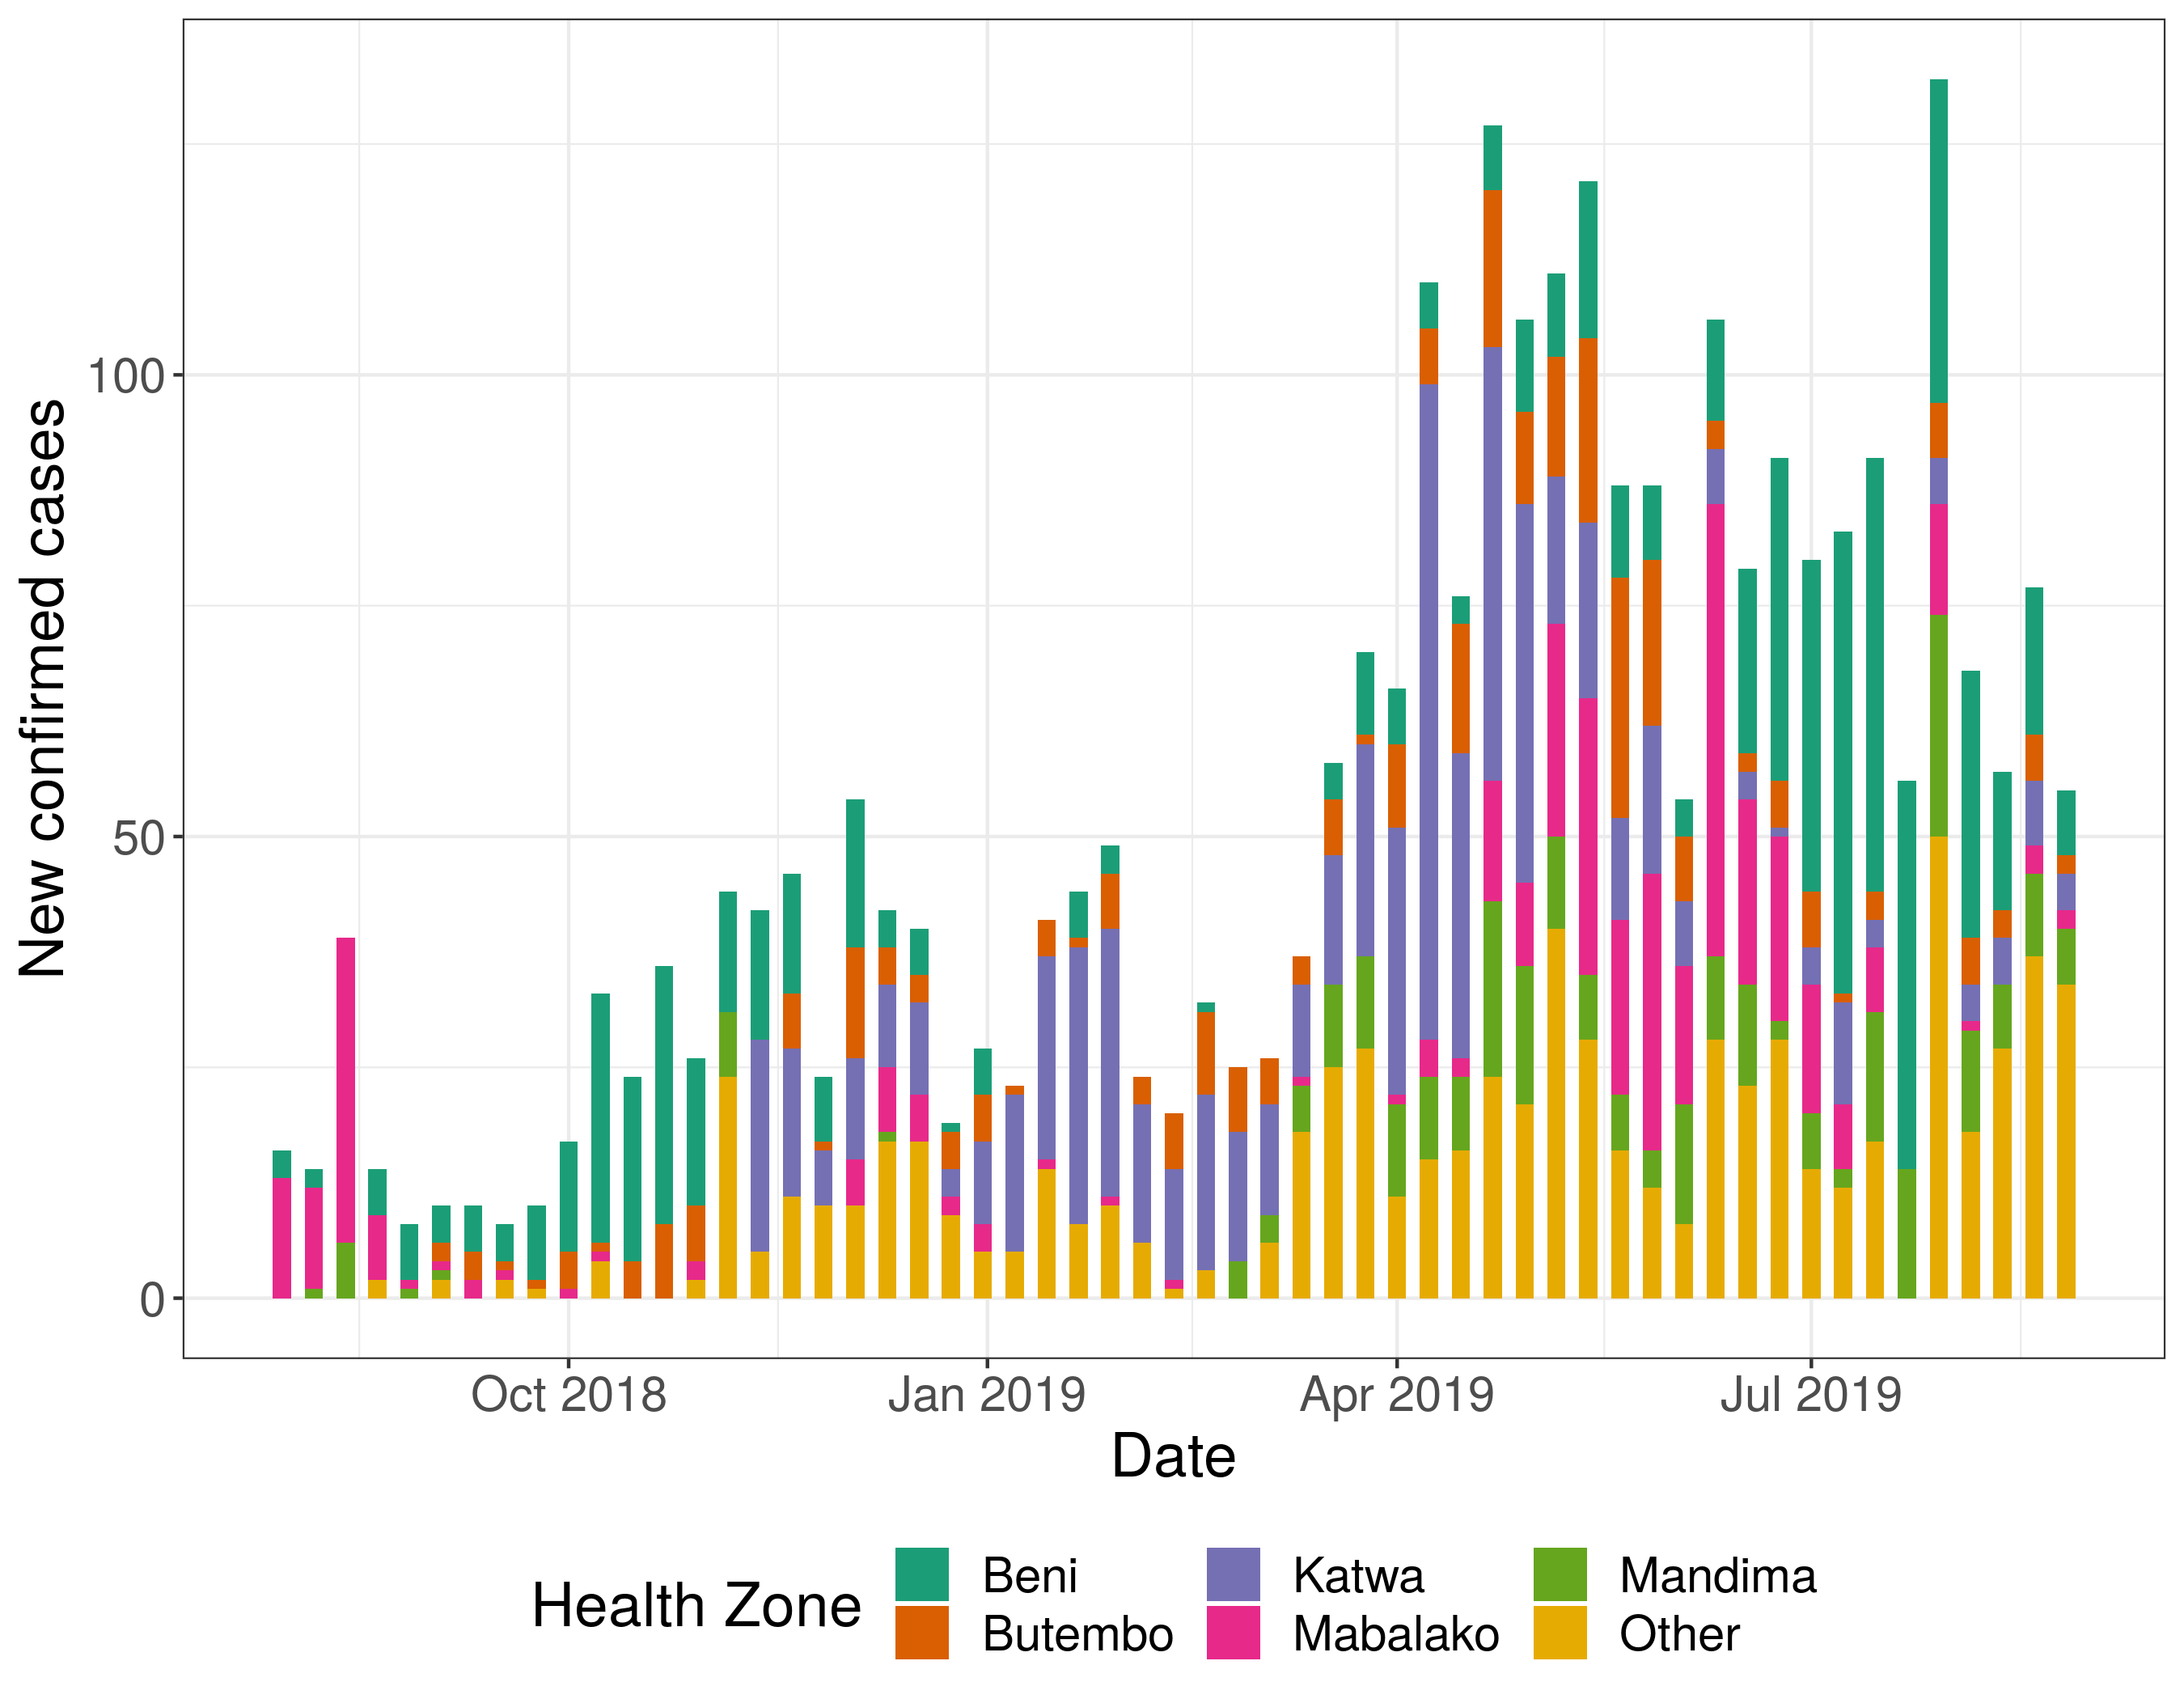
\includegraphics[width=\textwidth]{../output/epi_curve.png}
  \caption{Number of new confirmed cases by week in the health zones with the most Ebola Cases}
  \label{fig:epi_curve}
\end{subfigure}
\begin{subfigure}{0.48\textwidth}
  \centering
  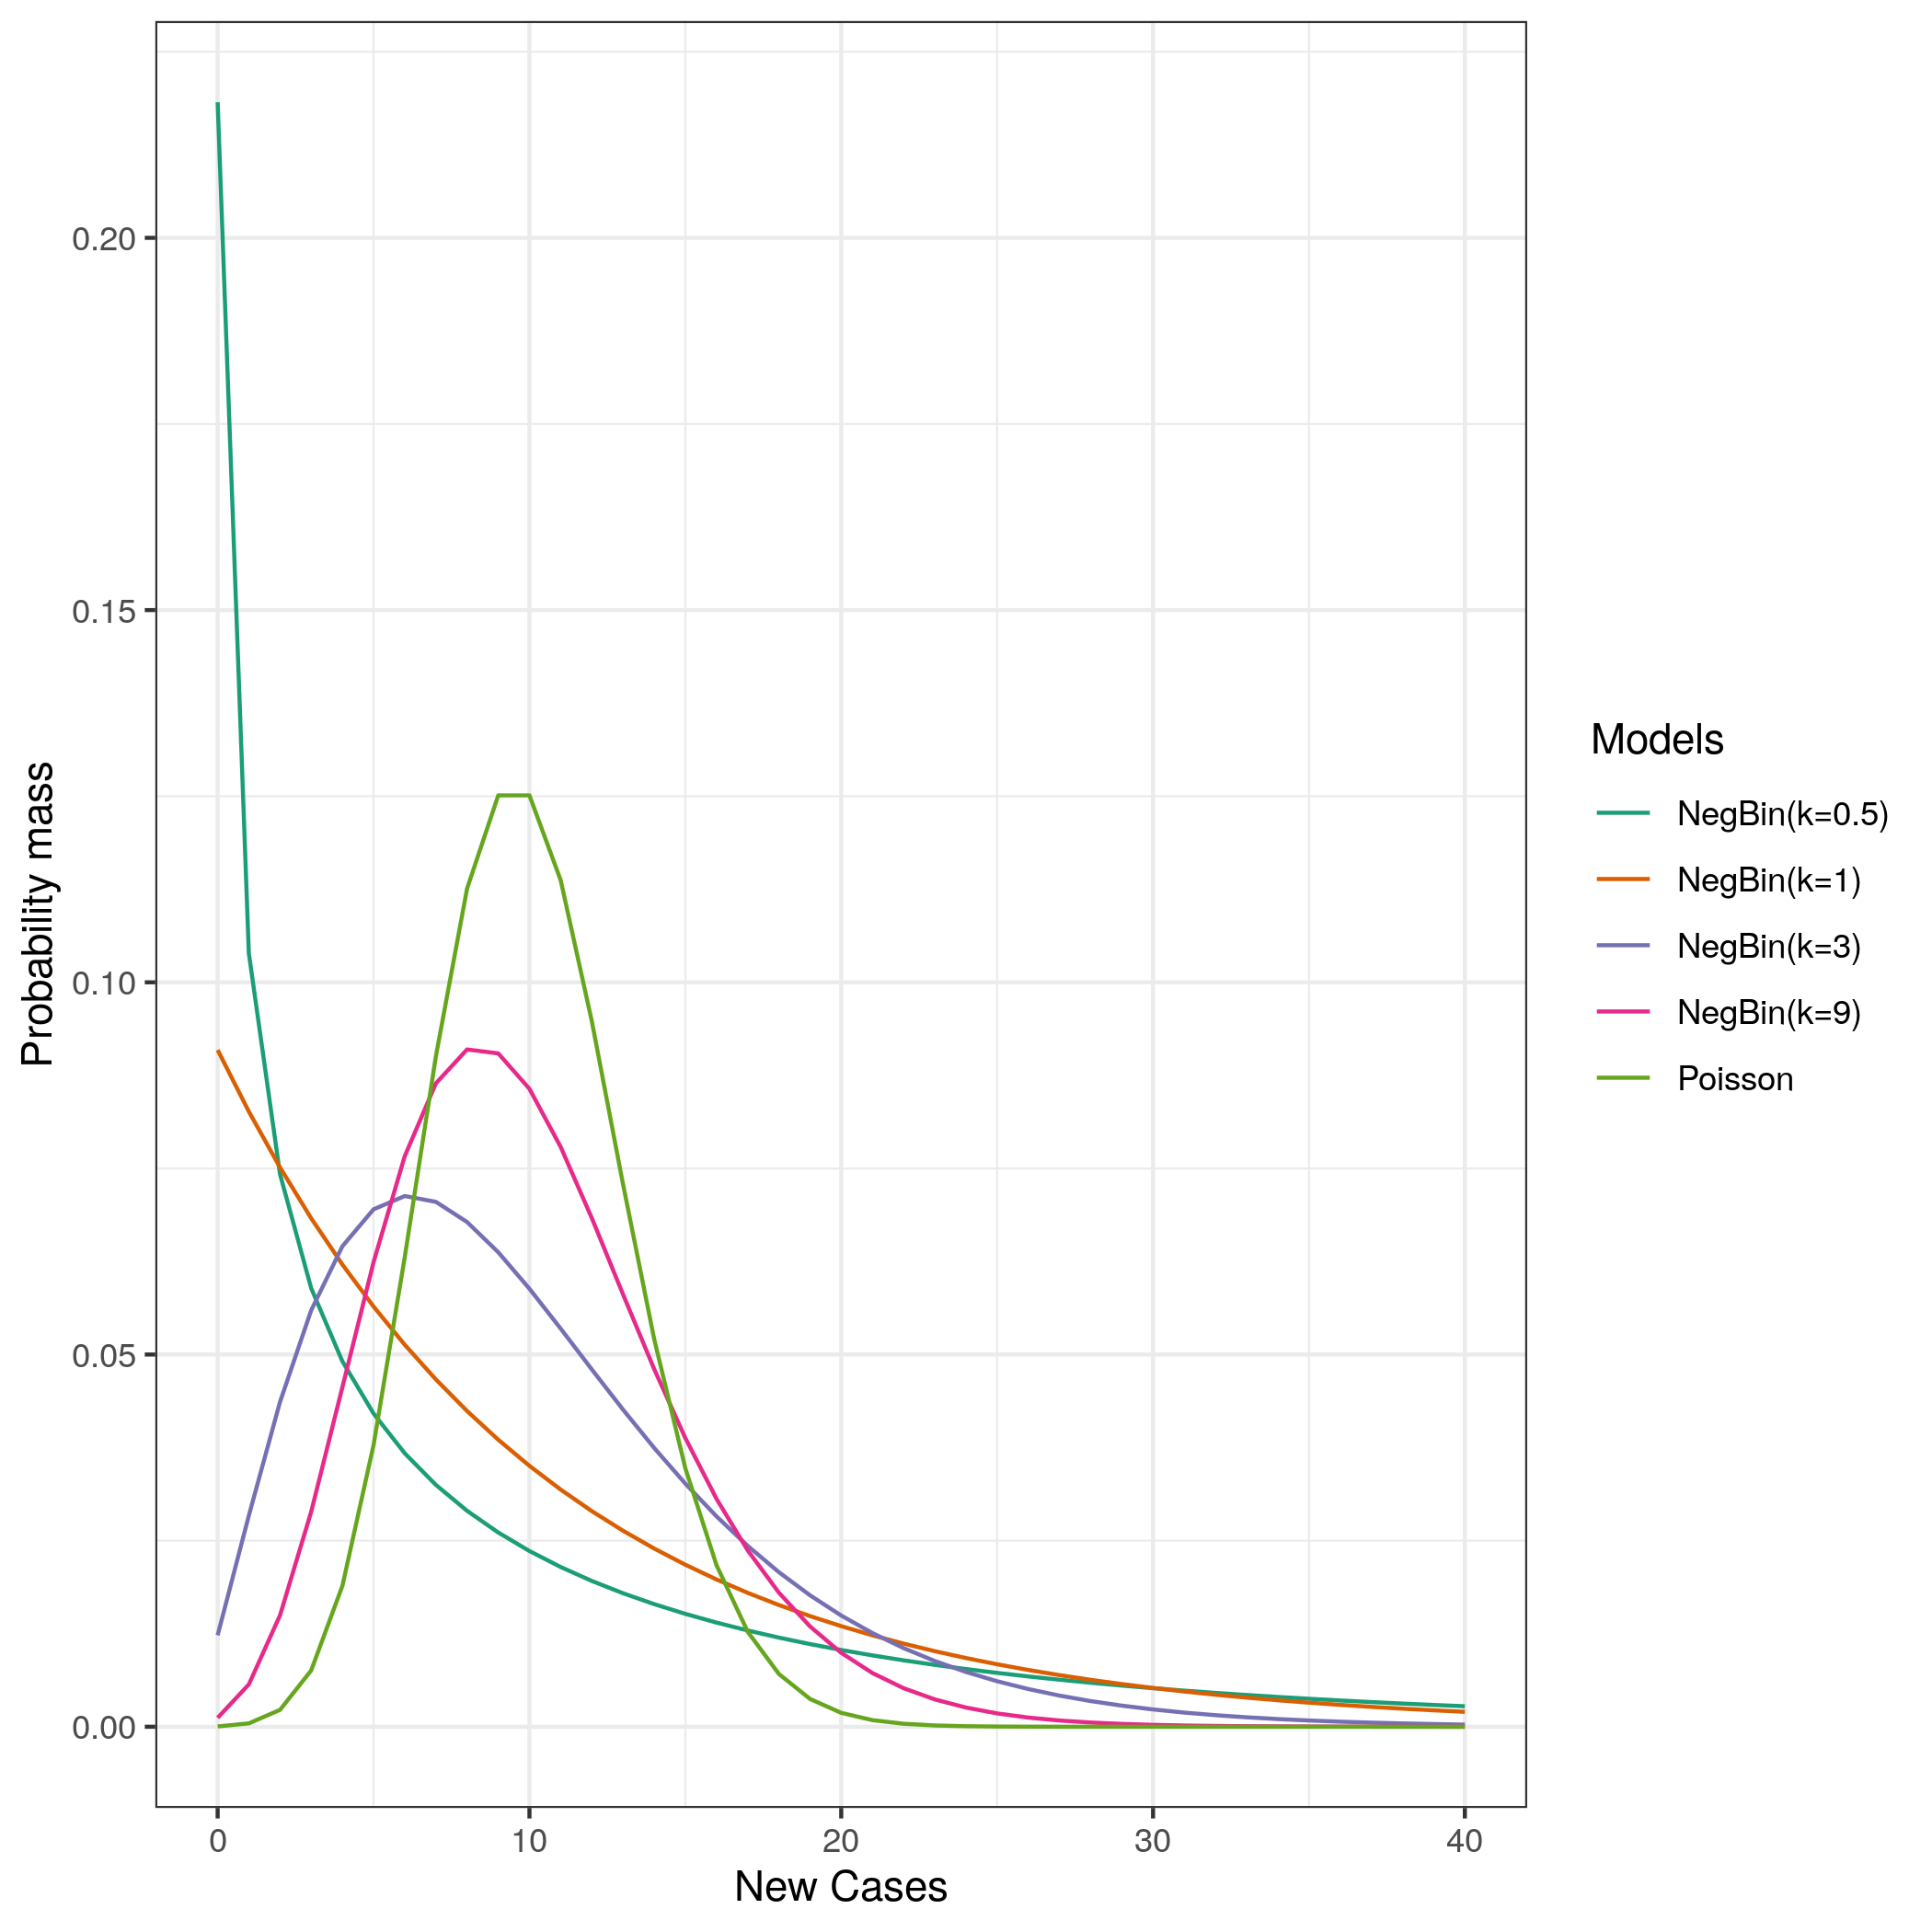
\includegraphics[height=5.7cm]{../output/tot_map.png}
  \caption{Total number of confirmed cases by Health Zone}
  \label{fig:tot_map}
\end{subfigure}

%% \bigskip

%% \begin{subfigure}{\textwidth}
%%   \centering
%%   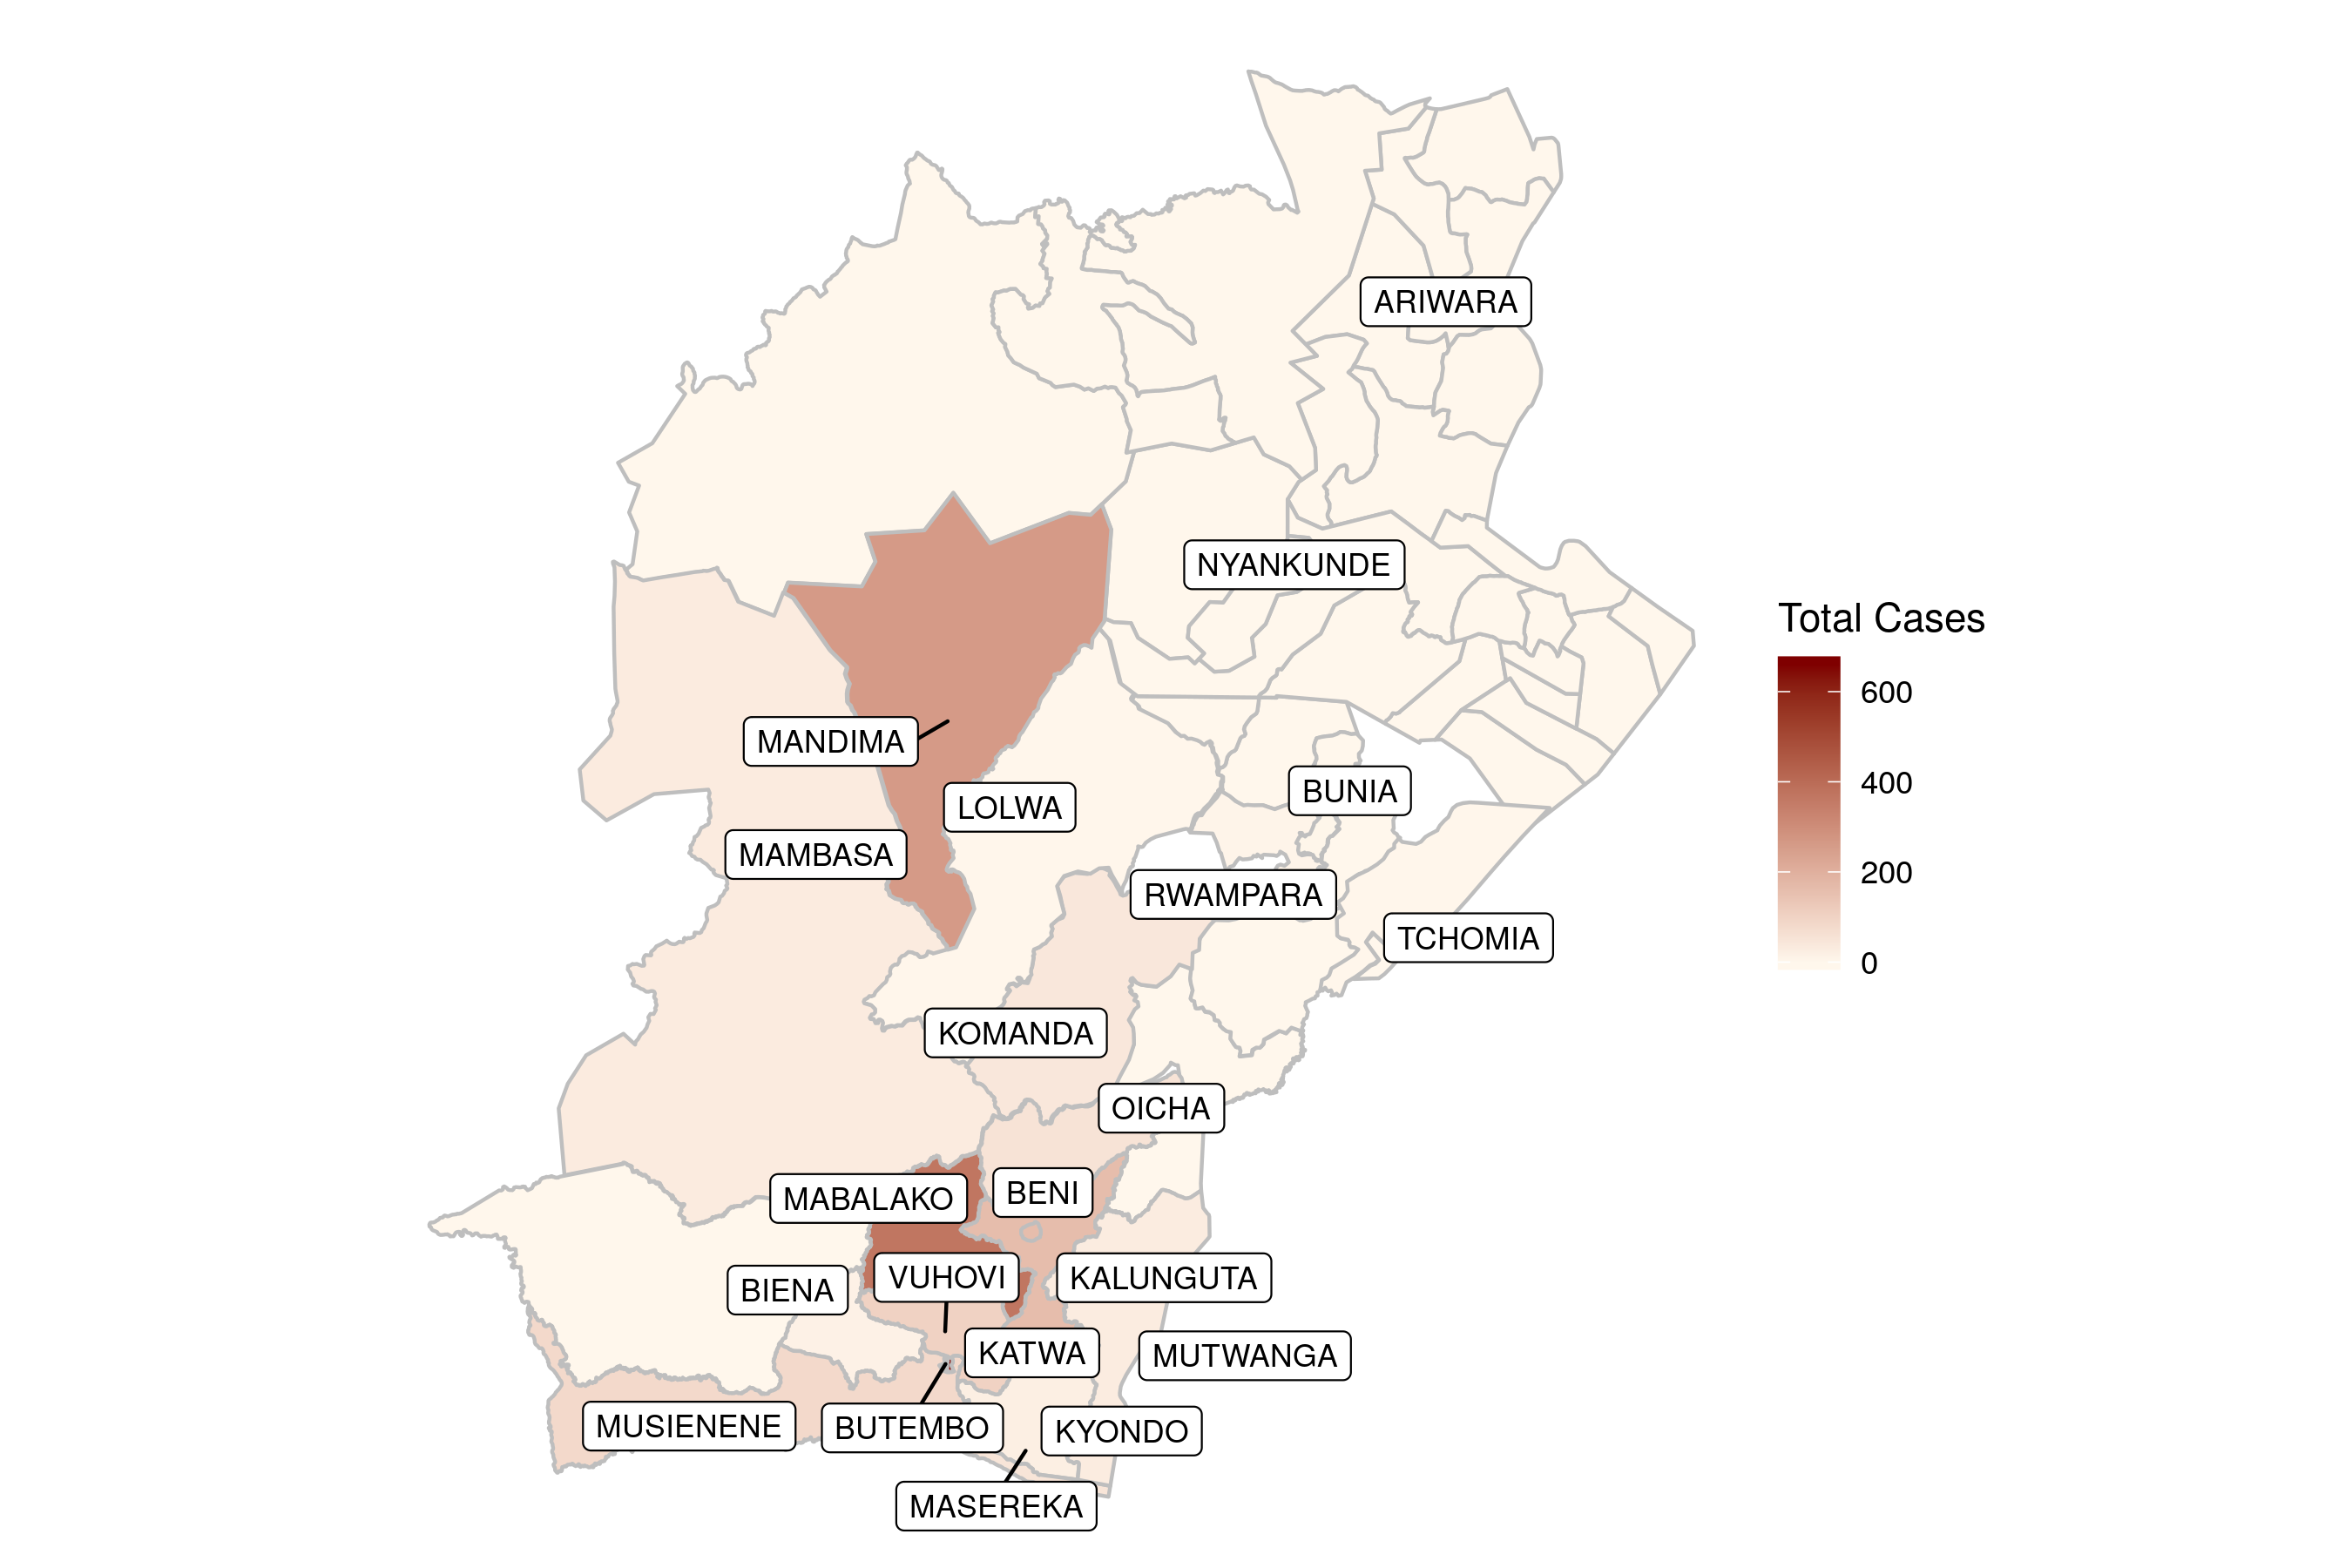
\includegraphics[width=0.7\textwidth]{../output/nat_rep.png}
%%   \caption{Reprodcution number as a function of time, the shaded region shows the 95\% credible interval}
%%   \label{fig:rep_num}
%% \end{subfigure}
\end{figure}

\subsection{National level forecasts}
We first found that the dispersion parameter that gives the smallest CRPS score for one day ahead predictions for the negative binomial models was k=8, but a fairly large range of parameters gave a reasonable fit. $k=8$ is  some more varriance than a poisson distribution, but much less than found in previous Ebola outbreaks as discussed above. 

All four models were sucesfully fitted on incidence data from 395 days and then used to provide short term forecasts. The calibration and proper scoring rules scores for the four models for different forecasting horizons can be seen in Table \ref{tab:nat_evo} for weekly forcasting horizons up to four weeks. We also show the the evolution of calibration, bias, CRPS and the centrality of PIT values as a function of the forecatsing horizon in Figure \ref{fig:nat_scores}
% latex table generated in R 3.6.1 by xtable 1.8-4 package
<<<<<<< HEAD
% Sat Sep  7 08:33:09 2019
=======
% Tue Sep 10 13:43:43 2019
>>>>>>> 6c96552641a3c339d41f2f58414064ece613e460
\begin{table}[ht]
\centering
\begin{tabular}{rlrrrrrrr}
  \hline
 & model & horizon & sharpness & bias & crps & dss & centrality & calibration \\ 
  \hline
<<<<<<< HEAD
1 & Negative Binomial Semilocal &   1 & 4.08 & -0.03 & 1.87 & 3.30 & 0.55 & 0.19 \\ 
  2 & Negative Binomial Latest &   1 & 4.14 & -0.00 & 1.82 & 3.26 & 0.56 & 0.17 \\ 
  3 & Poisson Semilocal &   1 & 2.93 & 0.01 & 1.87 & 3.32 & 0.43 & 0.00 \\ 
  4 & Poisson Latest &   1 & 2.97 & 0.05 & 1.82 & 3.24 & 0.42 & 0.00 \\ 
  5 & Negative Binomial Semilocal &   7 & 4.83 & -0.07 & 1.80 & 3.41 & 0.66 & 0.00 \\ 
  6 & Negative Binomial Latest &   7 & 4.33 & 0.01 & 2.36 & 3.94 & 0.47 & 0.00 \\ 
  7 & Poisson Semilocal &   7 & 4.19 & -0.02 & 1.72 & 3.23 & 0.59 & 0.01 \\ 
  8 & Poisson Latest &   7 & 3.08 & 0.06 & 2.47 & 4.31 & 0.36 & 0.00 \\ 
  9 & Negative Binomial Semilocal &  14 & 5.98 & -0.10 & 2.56 & 4.62 & 0.63 & 0.00 \\ 
  10 & Negative Binomial Latest &  14 & 4.62 & 0.02 & 2.82 & 4.74 & 0.41 & 0.00 \\ 
  11 & Poisson Semilocal &  14 & 5.78 & -0.06 & 2.52 & 4.54 & 0.60 & 0.00 \\ 
  12 & Poisson Latest &  14 & 3.28 & 0.09 & 2.99 & 5.32 & 0.29 & 0.00 \\ 
  13 & Negative Binomial Semilocal &  21 & 7.55 & -0.13 & 3.24 & 5.69 & 0.65 & 0.00 \\ 
  14 & Negative Binomial Latest &  21 & 5.12 & 0.01 & 4.07 & 5.57 & 0.31 & 0.00 \\ 
  15 & Poisson Semilocal &  21 & 7.67 & -0.10 & 3.26 & 5.88 & 0.65 & 0.00 \\ 
  16 & Poisson Latest &  21 & 3.53 & 0.06 & 4.54 & 6.85 & 0.24 & 0.00 \\ 
  17 & Negative Binomial Semilocal &  28 & 9.14 & -0.16 & 4.77 & 7.43 & 0.67 & 0.00 \\ 
  18 & Negative Binomial Latest &  28 & 5.87 & 0.03 & 5.30 & 7.38 & 0.30 & 0.00 \\ 
  19 & Poisson Semilocal &  28 & 9.64 & -0.13 & 4.89 & 7.12 & 0.66 & 0.00 \\ 
  20 & Poisson Latest &  28 & 3.88 & 0.08 & 6.00 & 9.08 & 0.22 & 0.00 \\ 
=======
1 & Negative Binomial Semilocal &   1 & 4.08 & -0.65 & 1.87 & 3.30 & 0.05 & 0.19 \\ 
  2 & Negative Binomial Latest &   1 & 4.14 & -0.65 & 1.82 & 3.26 & 0.06 & 0.16 \\ 
  3 & Poisson Semilocal &   1 & 2.93 & -0.65 & 1.87 & 3.32 & -0.07 & 0.00 \\ 
  4 & Poisson Latest &   1 & 2.97 & -0.65 & 1.82 & 3.24 & -0.08 & 0.00 \\ 
  5 & Negative Binomial Semilocal &   7 & 4.83 & -0.65 & 1.80 & 3.41 & 0.16 & 0.00 \\ 
  6 & Negative Binomial Latest &   7 & 4.33 & -0.65 & 2.36 & 3.94 & -0.04 & 0.00 \\ 
  7 & Poisson Semilocal &   7 & 4.19 & -0.65 & 1.72 & 3.23 & 0.09 & 0.01 \\ 
  8 & Poisson Latest &   7 & 3.08 & -0.65 & 2.47 & 4.31 & -0.14 & 0.00 \\ 
  9 & Negative Binomial Semilocal &  14 & 5.98 & -0.66 & 2.56 & 4.62 & 0.14 & 0.00 \\ 
  10 & Negative Binomial Latest &  14 & 4.62 & -0.66 & 2.82 & 4.74 & -0.08 & 0.00 \\ 
  11 & Poisson Semilocal &  14 & 5.78 & -0.66 & 2.52 & 4.54 & 0.10 & 0.00 \\ 
  12 & Poisson Latest &  14 & 3.28 & -0.66 & 2.99 & 5.32 & -0.21 & 0.00 \\ 
  13 & Negative Binomial Semilocal &  21 & 7.55 & -0.67 & 3.24 & 5.69 & 0.15 & 0.00 \\ 
  14 & Negative Binomial Latest &  21 & 5.12 & -0.67 & 4.07 & 5.57 & -0.19 & 0.00 \\ 
  15 & Poisson Semilocal &  21 & 7.67 & -0.67 & 3.26 & 5.88 & 0.16 & 0.00 \\ 
  16 & Poisson Latest &  21 & 3.53 & -0.67 & 4.54 & 6.85 & -0.26 & 0.00 \\ 
  17 & Negative Binomial Semilocal &  28 & 9.14 & -0.68 & 4.77 & 7.43 & 0.17 & 0.00 \\ 
  18 & Negative Binomial Latest &  28 & 5.87 & -0.68 & 5.30 & 7.38 & -0.20 & 0.00 \\ 
  19 & Poisson Semilocal &  28 & 9.64 & -0.68 & 4.89 & 7.12 & 0.16 & 0.00 \\ 
  20 & Poisson Latest &  28 & 3.88 & -0.68 & 6.00 & 9.08 & -0.28 & 0.00 \\ 
>>>>>>> 6c96552641a3c339d41f2f58414064ece613e460
   \hline
\end{tabular}
\caption{Model evaluations for predictions when all the models are fitted on the combined data from all the health zones.} 
\label{tab:nat_evo}
\end{table}



\begin{figure}[h]
\begin{subfigure}{\textwidth}
  \centering
  % include first image
  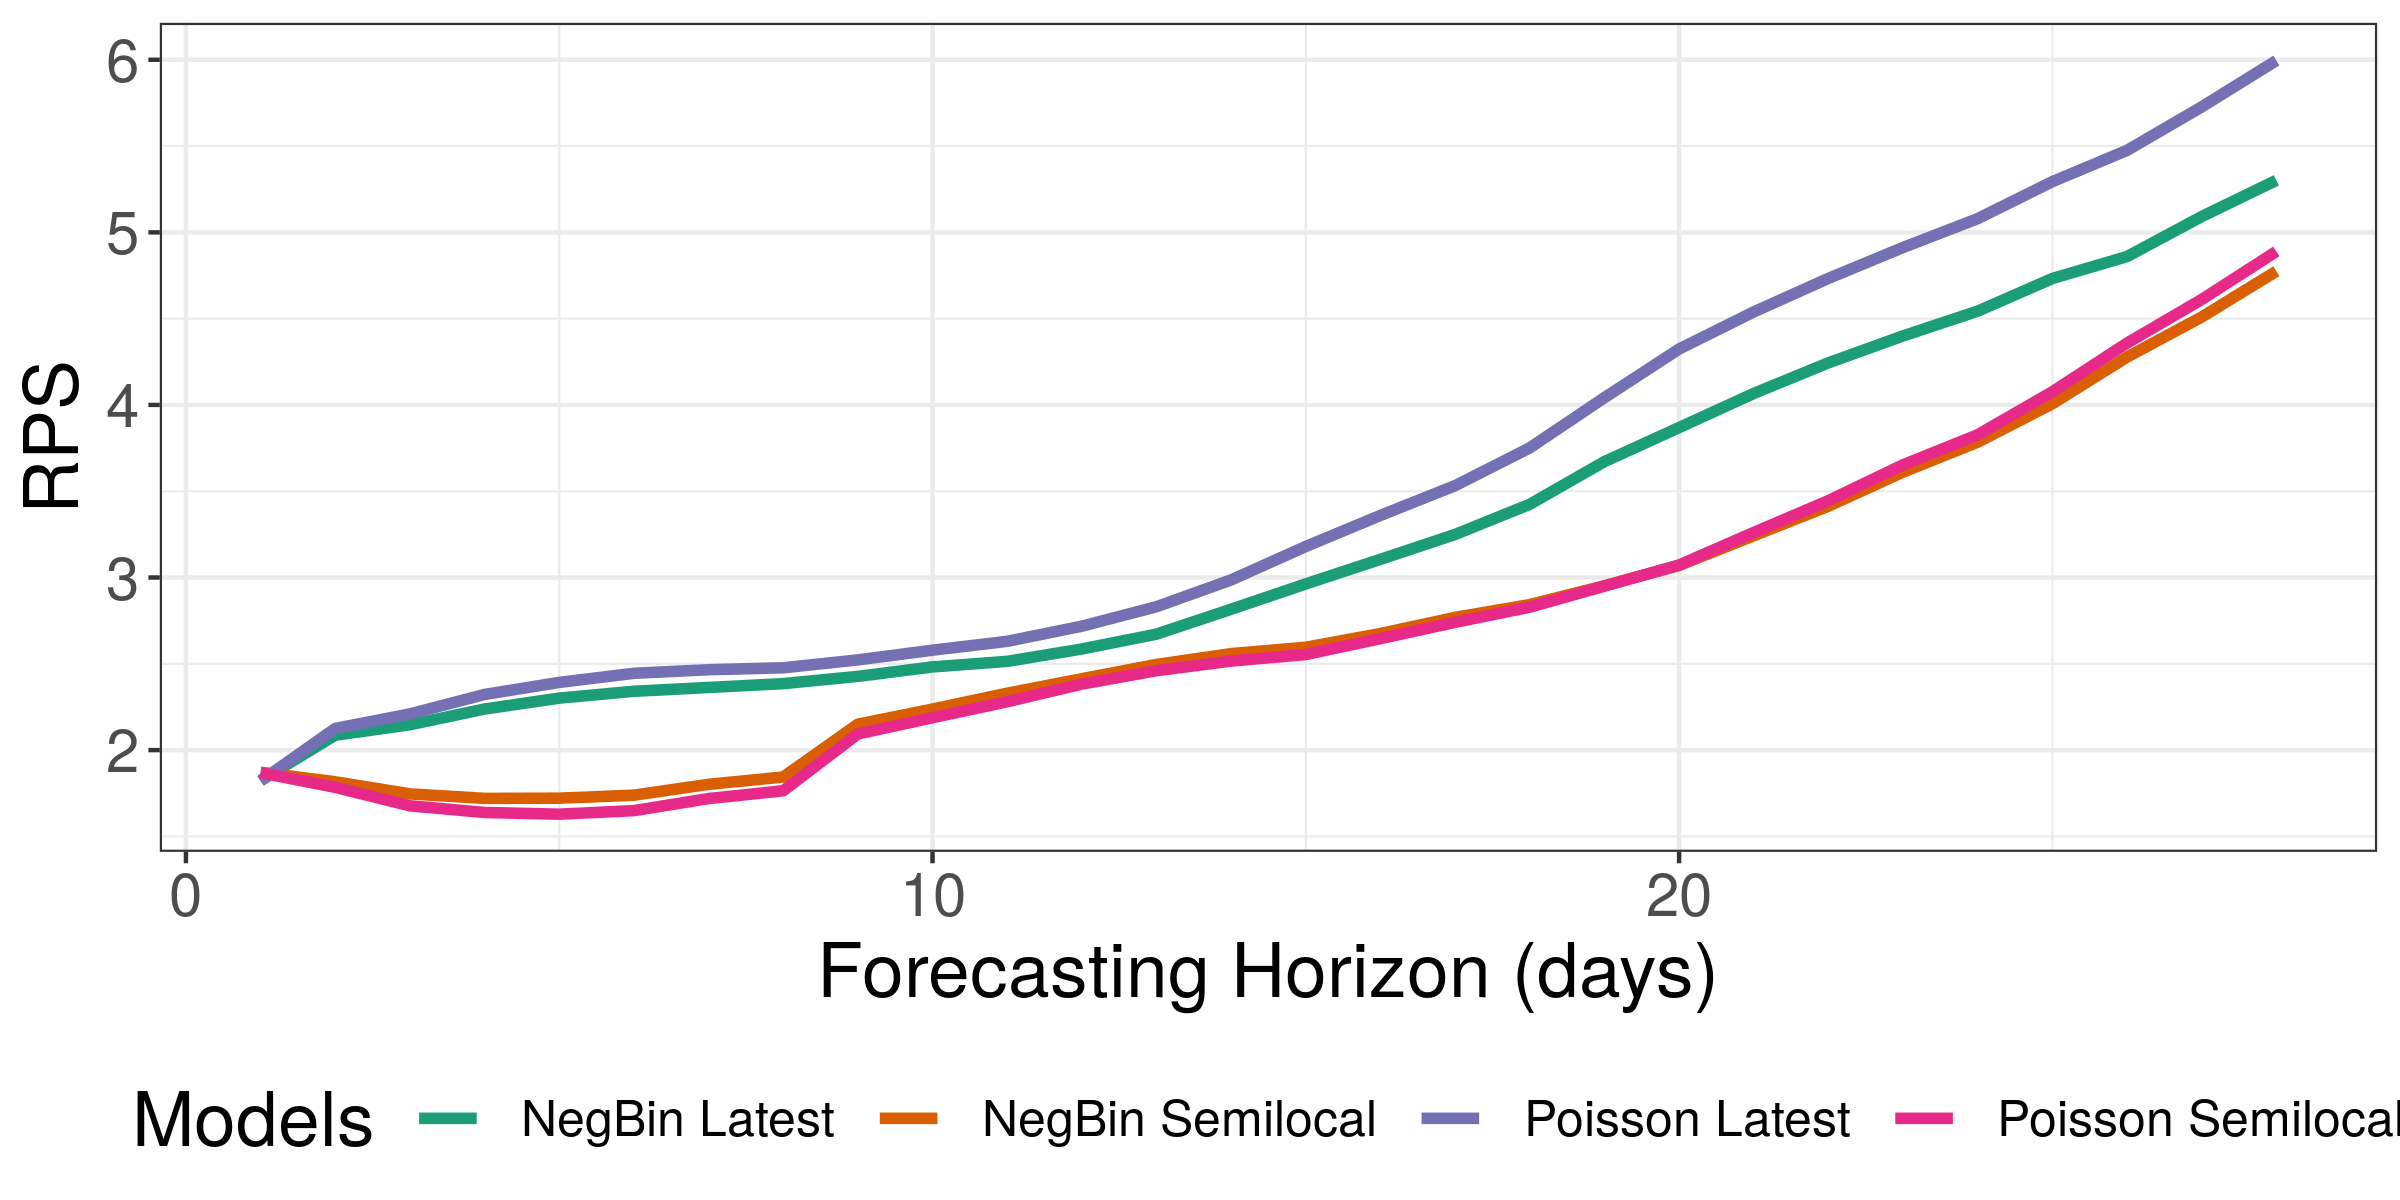
\includegraphics[width=0.9\linewidth]{../output/national_crps.png}  
  \caption{Contineously Ranked Probability Score}
  \label{fig:sub-first}
\end{subfigure}

\begin{subfigure}{\textwidth}
  \centering
  % include second image
  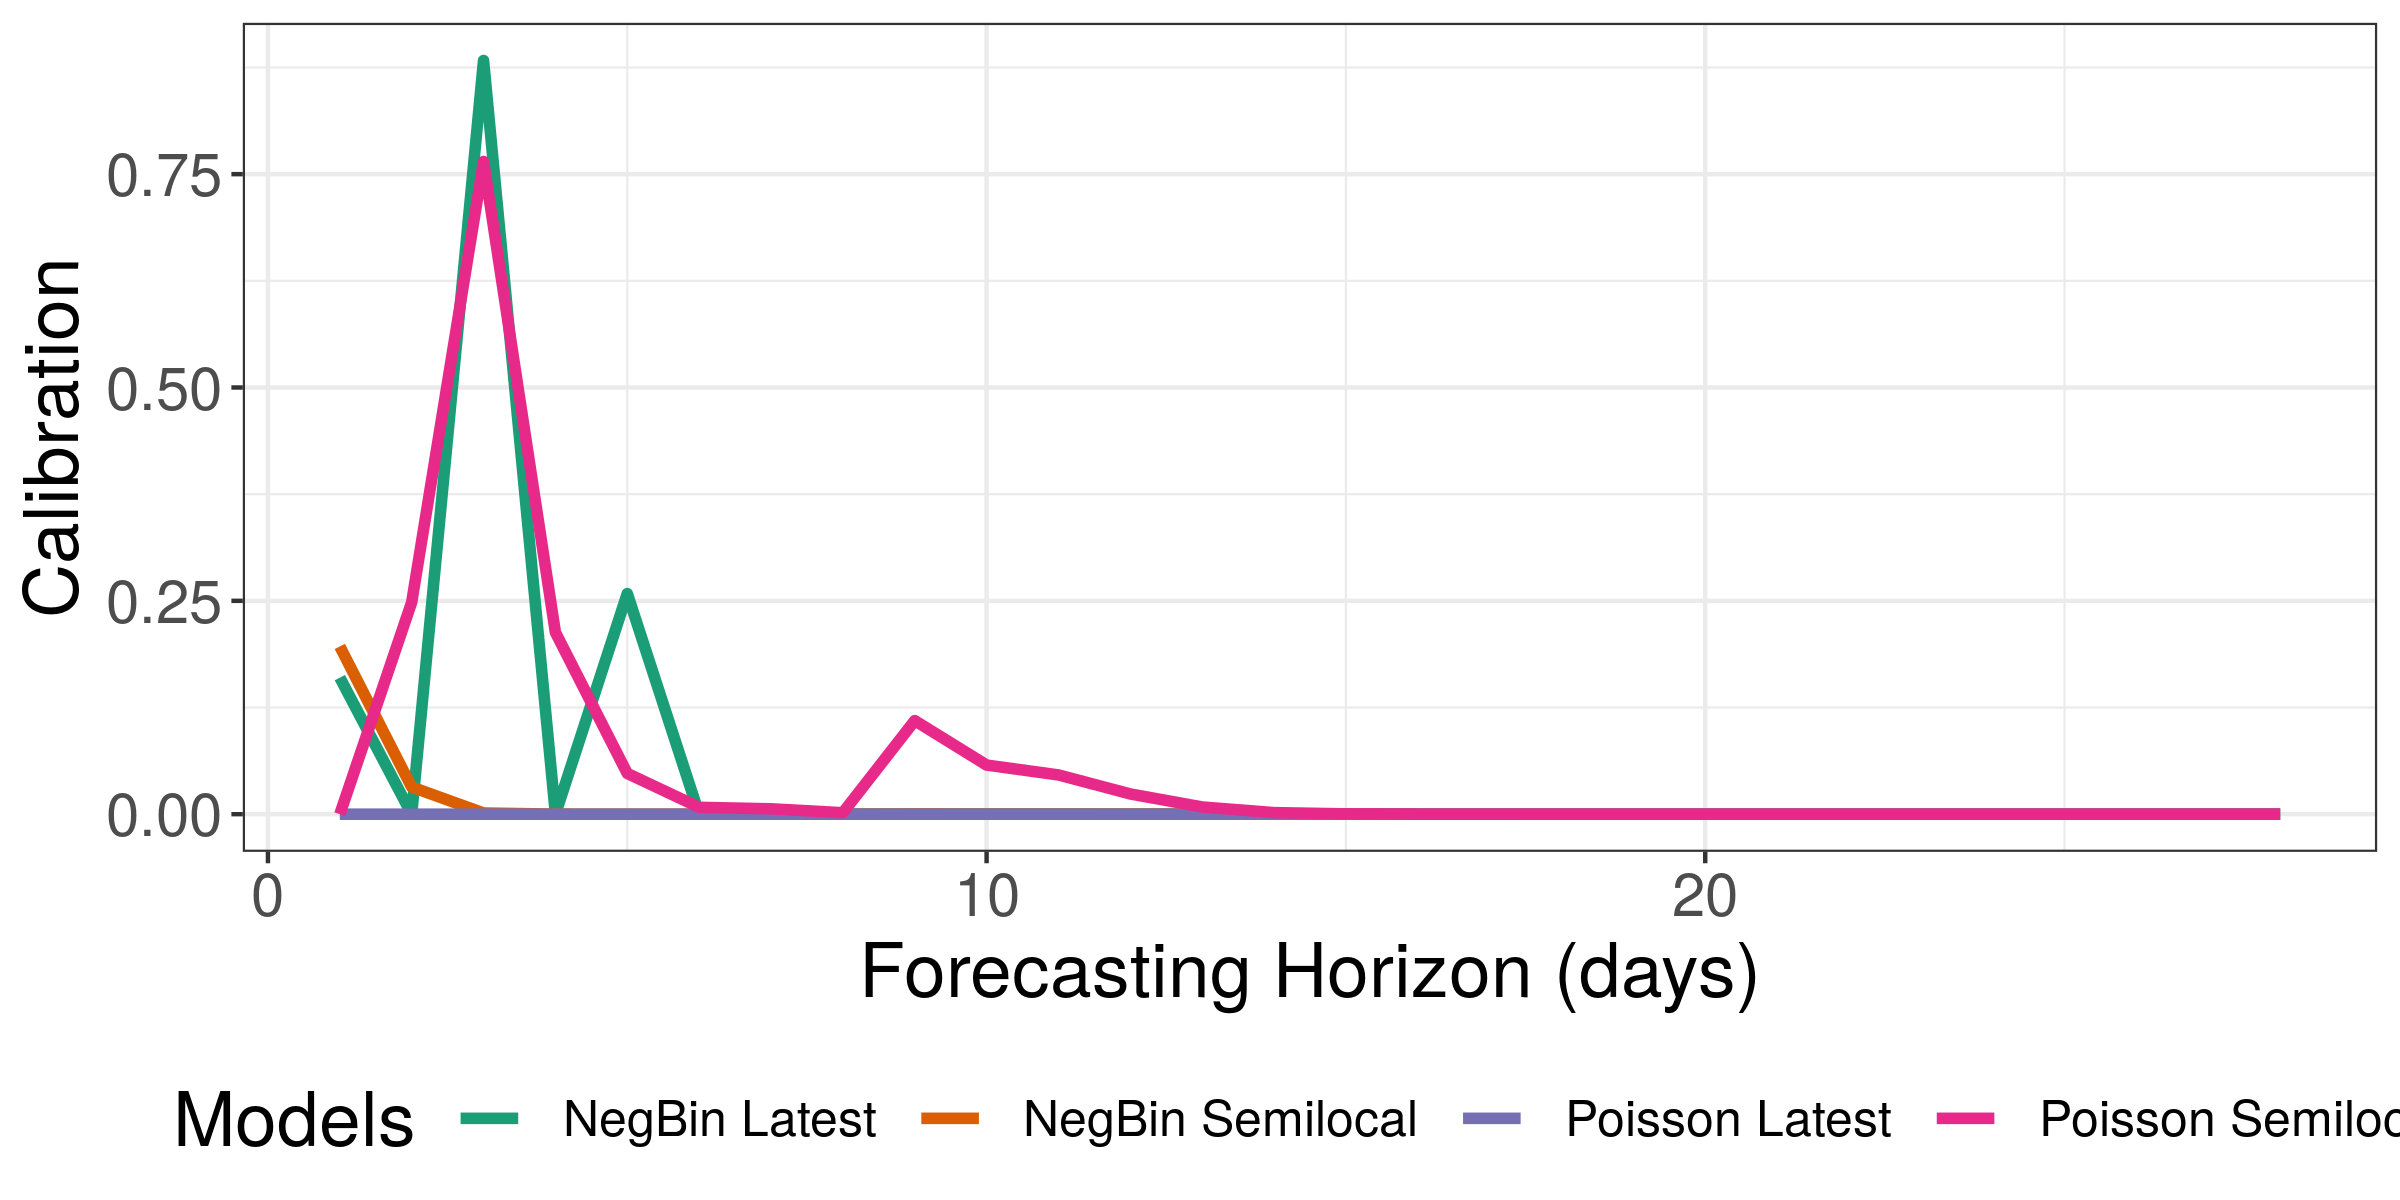
\includegraphics[width=0.9\linewidth]{../output/national_calibration.png}  
  \caption{Calibration p-value}
  \label{fig:sub-second}
\end{subfigure}
\begin{subfigure}{\textwidth}
  \centering
  % include second image
  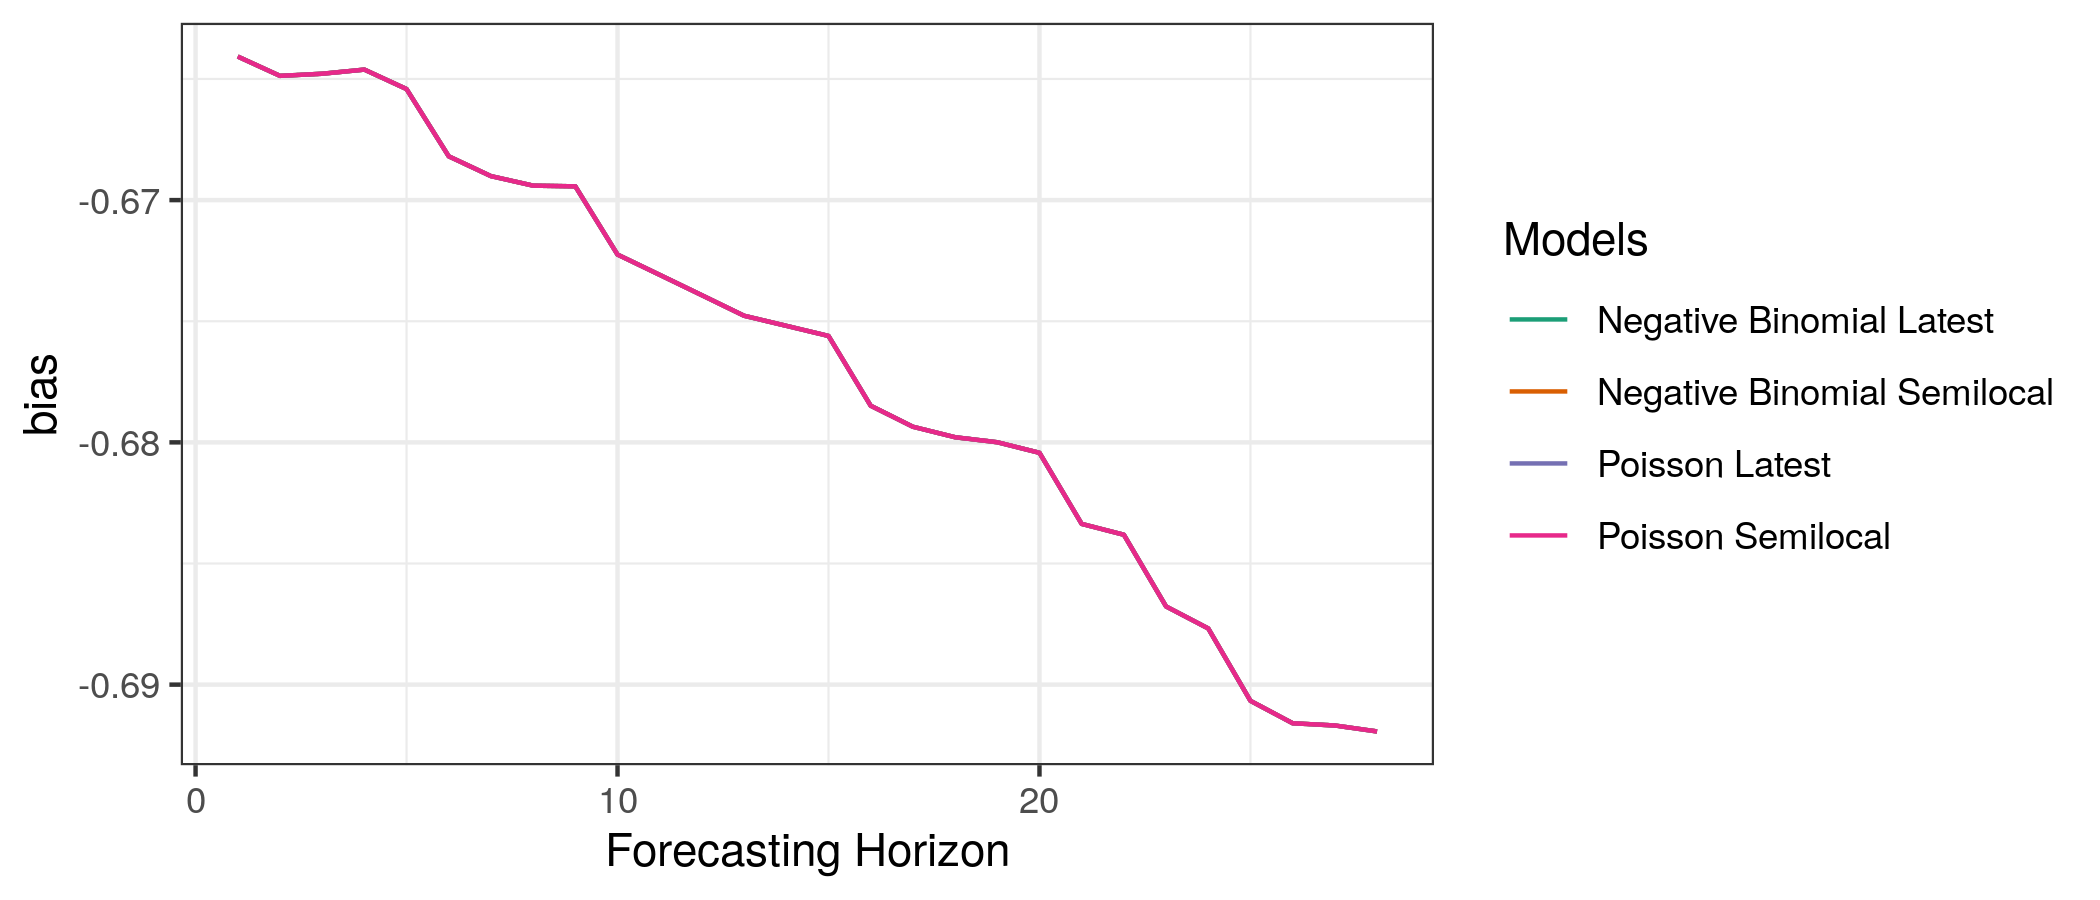
\includegraphics[width=0.9\linewidth]{../output/national_bias.png}  
  \caption{Bias}
  \label{fig:sub-third}
\end{subfigure}
\begin{subfigure}{\textwidth}
  \centering
  % include second image
  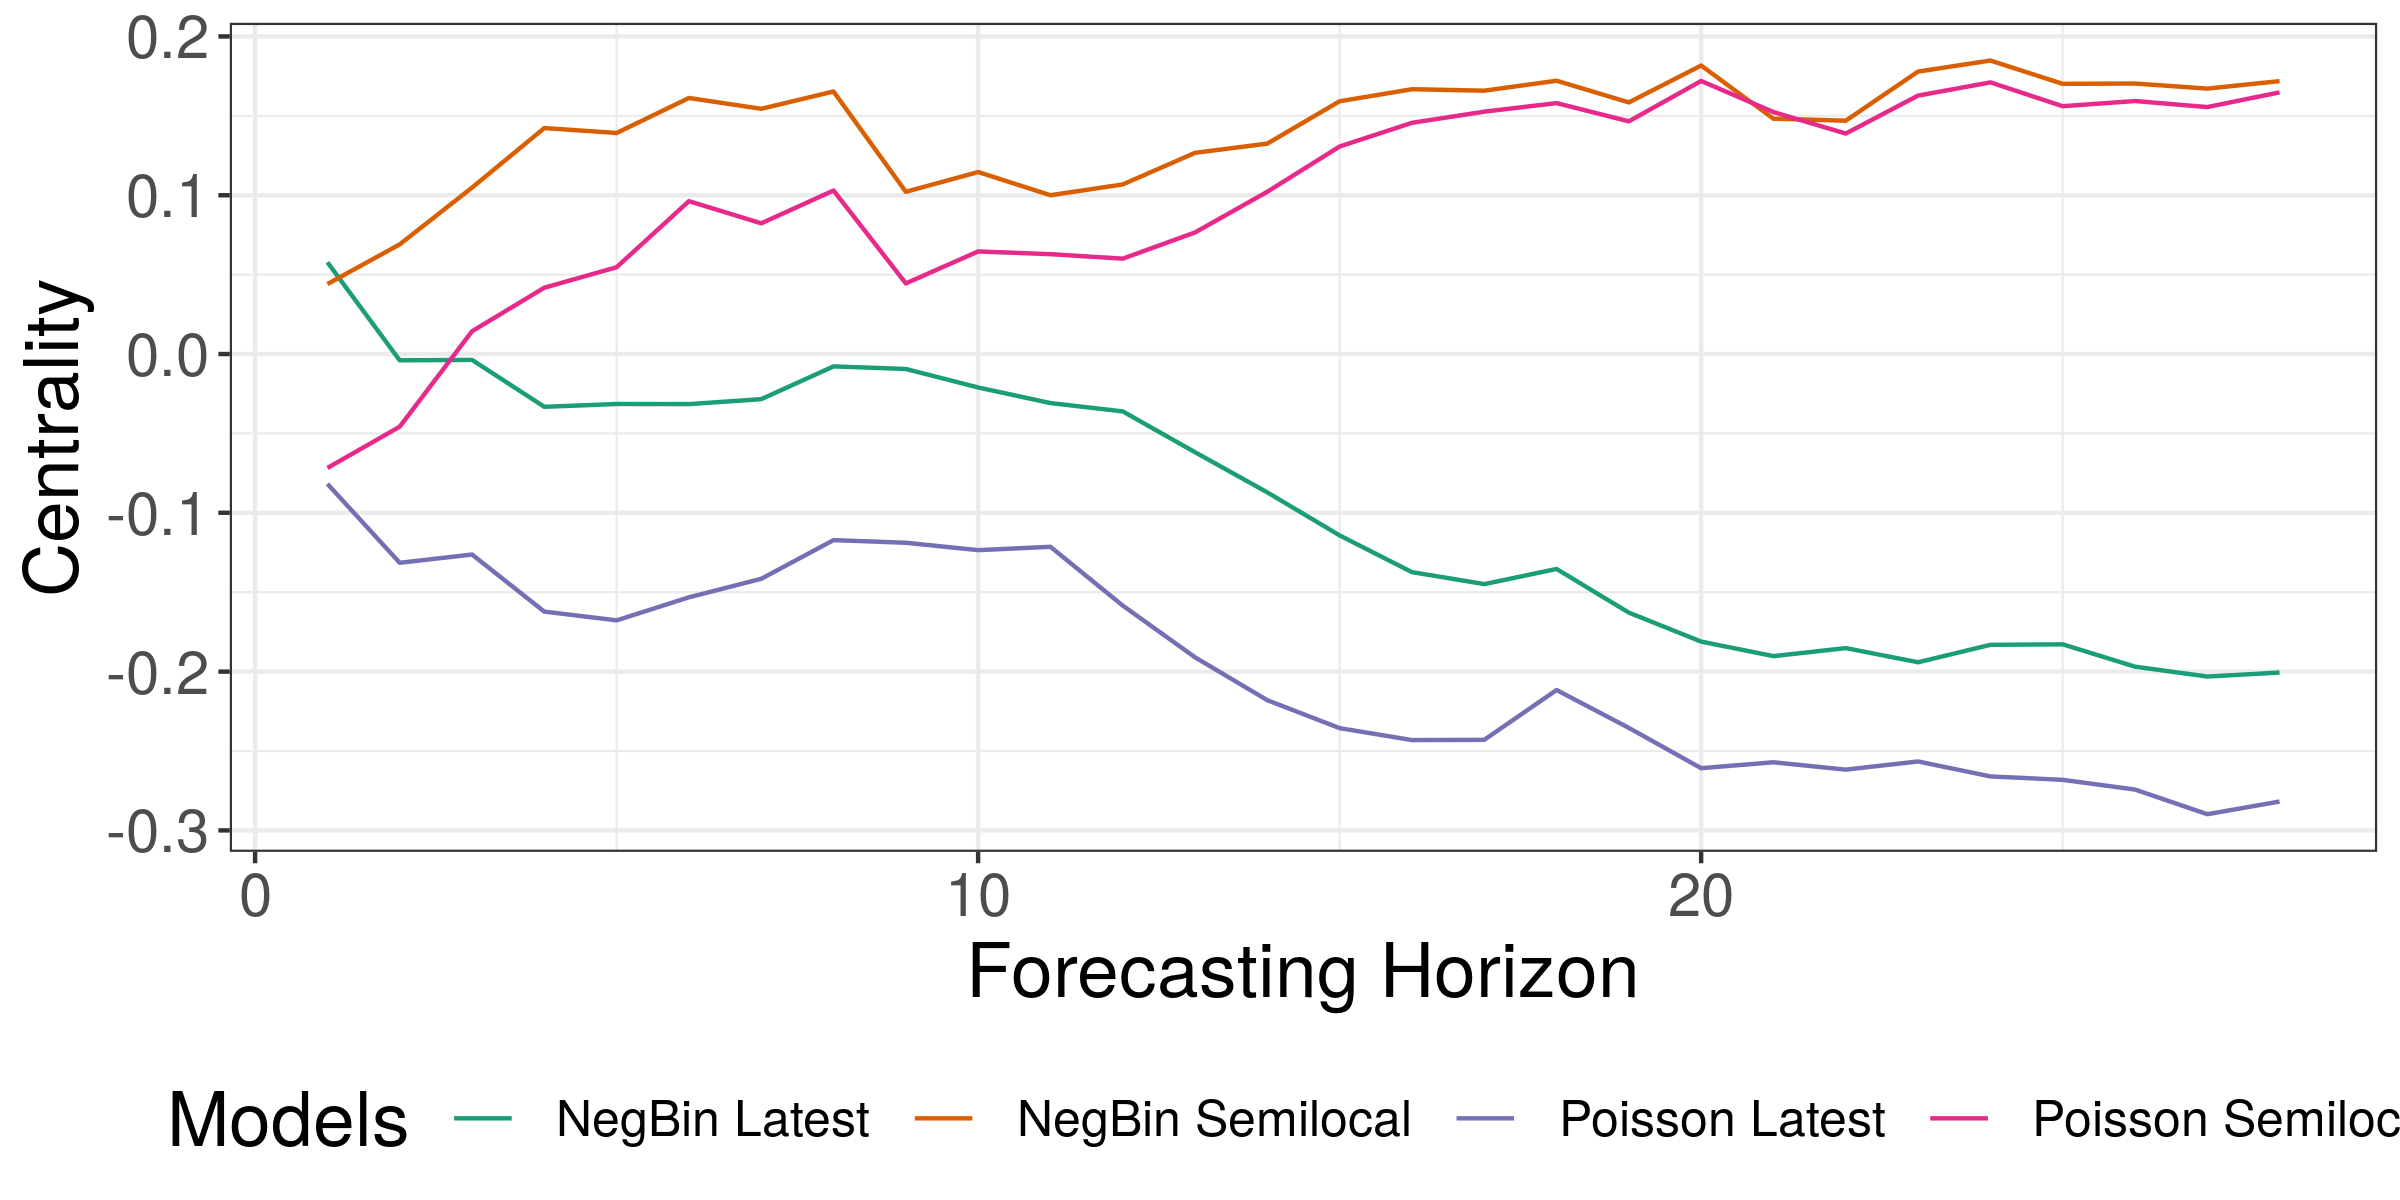
\includegraphics[width=0.9\linewidth]{../output/national_centrality.png}  
  \caption{Centrality of PIT values}
  \label{fig:sub-fourth}
\end{subfigure}
  \caption{Scores for the entire outbreak as a function of the forecasting horizon.}

  \label{fig:nat_scores}
\end{figure}

Together they show that for next day forecast, the negative binomial offspring distirbution is needed for a calibrated forecast. The negative binomial distribution is clearly needed for a calibrated forecast even for one day ahead predictions. For longer forecasting horizons the poisson distribution with the semilocal time series prediction for $R_t$ is the best model and is calibrated out to about 12 days. From the centrality scores, we can see that both the models with time series are overestimating the dispersion and the negative binomial model more so than the poisson model. Based on the scoring rules the two time series models are signficantly better than the models without any evaluation in $R_t$.

To understand the local poisson model better we calculate 28 day forecasts every 50 days of the outbreak and compared those forecasted incidence values with observed values. This can be seen in Figure \ref{fig:nat_pred}. In the same figure we also plot the estimated values of the reproduction number together with 28 day forecasts for the same model. We see reasonable predictions, especially in the short term. We also here see that the model probably overestimates the uncertainty in both the reproduction number and the incidence. 
\begin{figure}[h]
\begin{subfigure}{\textwidth}
  \centering
  % include first image
  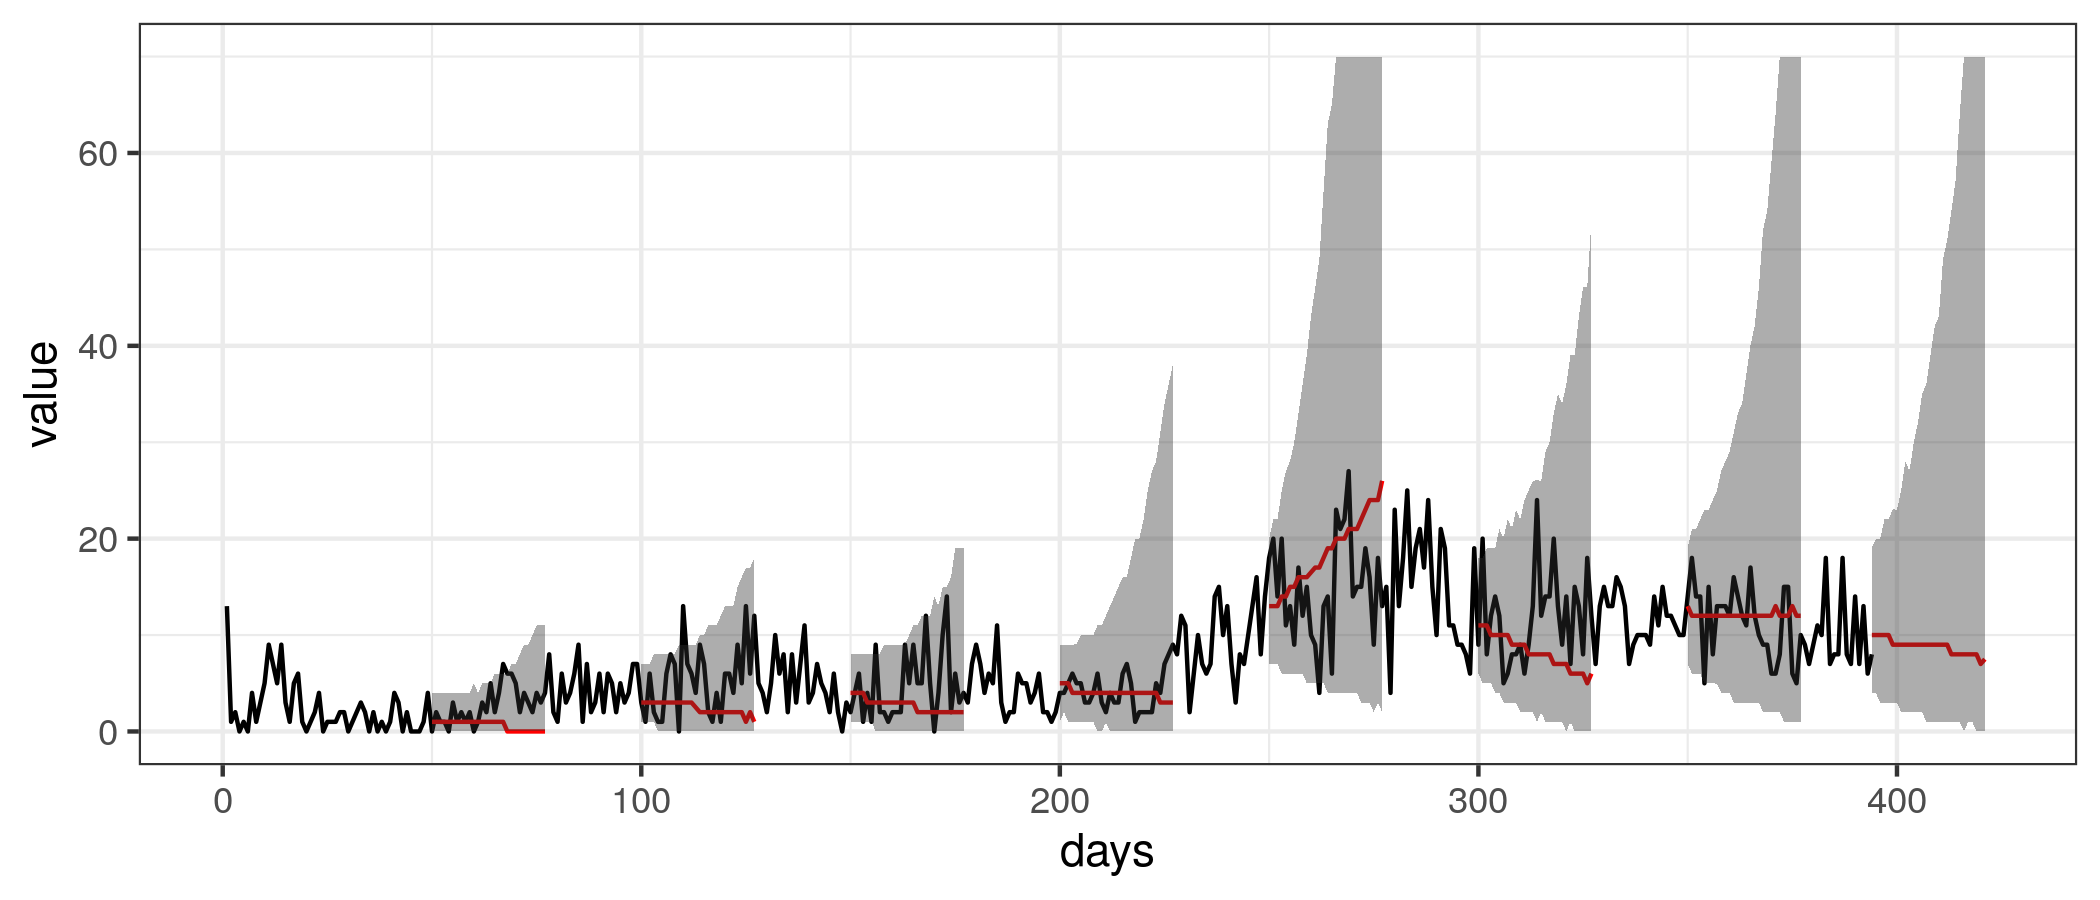
\includegraphics[width=0.9\linewidth]{../output/national_predictions.png}  
  \caption{Forecasted and predicted incidence for the semilocal poisson model}
  \label{fig:sub-first}
\end{subfigure}

\begin{subfigure}{\textwidth}
  \centering
  % include second image
  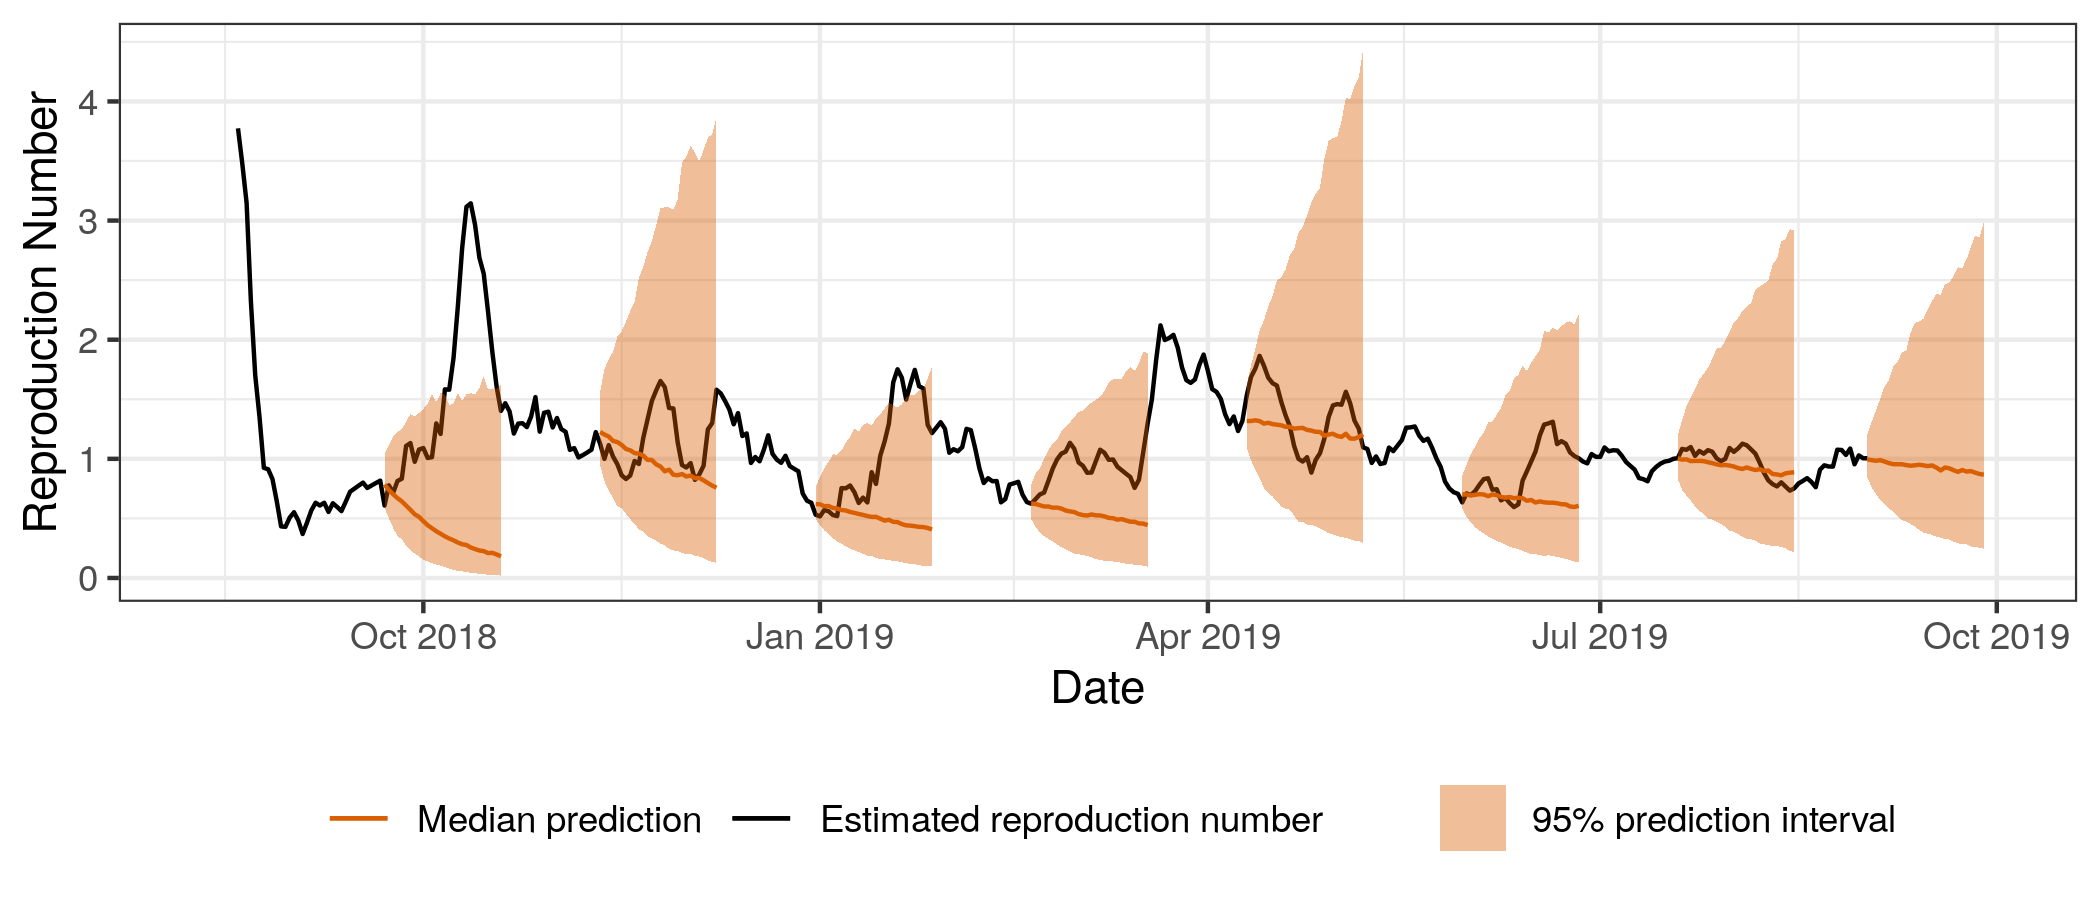
\includegraphics[width=0.9\linewidth]{../output/national_Rs.png}  
  \caption{Forecasted and predicted repreoduction numbers for the semilocal poisson model}
  \label{fig:sub-second}
\end{subfigure}
  \caption{Median forecast with 95\% prediction intervals and observed values for incidence and reproduction number for the semilocal poisson model}.

  \label{fig:nat_pred}
\end{figure}







\subsection{Health Zones}

%% The averaged evaluations when we predicted the future incidence for individual health zones can be seen in Table \ref{tab:hz_evo}.
 % latex table generated in R 3.6.1 by xtable 1.8-4 package
% Tue Sep 24 17:36:32 2019
\begin{table}[h!]
\centering
\begin{tabular}{|l|l|l|l|}
  \hline
Location & Largest Horizon & Best model & Cases \\ 
  \hline
Kayna & 28 & NegBin Semilocal & 22 \\ 
  Nyiragongo & 28 & NegBin Semilocal & 3 \\ 
  Tchomia & 28 & NegBin Semilocal & 2 \\ 
  Lolwa & 26 & All models & 3 \\ 
  Mwenga & 18 & All models & 6 \\ 
  Bunia & 17 & NegBin Semilocal & 4 \\ 
  Alimbongo & 12 & NegBin Semilocal & 5 \\ 
  national & 9 & Poisson Semilocal & 2942 \\ 
  Kayina & 7 & Poisson Semilocal & 10 \\ 
  Rwampara & 6 & NegBin Latest & 8 \\ 
  Lubero & 4 & NegBin Semilocal & 31 \\ 
  Musienene & 4 & Poisson Semilocal & 84 \\ 
  Kyondo & 3 & Poisson Semilocal & 22 \\ 
  Vuhovi & 3 & Poisson Semilocal & 103 \\ 
  Beni & 2 & Poisson Semilocal & 661 \\ 
  Biena & 2 & Poisson Latest & 16 \\ 
  Butembo & 2 & NegBin Semilocal & 279 \\ 
  Mabalako & 2 & NegBin Semilocal & 371 \\ 
  Kalunguta & NA & No calibrated model & 164 \\ 
  Katwa & NA & No calibrated model & 647 \\ 
  Mangurujipa & NA & No calibrated model & 20 \\ 
  Masereka & NA & No calibrated model & 50 \\ 
  Mutwanga & NA & No calibrated model & 31 \\ 
  Oicha & NA & No calibrated model & 55 \\ 
  Komanda & NA & No calibrated model & 43 \\ 
  Mambasa & NA & No calibrated model & 32 \\ 
  Mandima & NA & No calibrated model & 264 \\ 
   \hline
\end{tabular}
\caption{For each health zone we show the maximal forecasting horizon where we can not exclude calibration at the p=0.1 level. If multiple models are equally calibrated we chosse the one with smallest RPS. For some health zones there were no calibrated forecasts} 
\label{tab:best_model}
\end{table}


%% Evaluations for each health zone for the Poisson Semilocal model in Table \ref{tab:by_hz_evo}.
%% % latex table generated in R 3.6.1 by xtable 1.8-4 package
% Tue Sep 10 13:44:08 2019
\begin{table}[ht]
\centering
\begin{tabular}{rlrrrrrrrr}
  \hline
 & location & horizon & crps & dss & calibration & centrality & sharpness & bias & cases \\ 
  \hline
1 & Tchomia &   7 & 0.00 &  & 0.52 & 0.02 & 0.00 & 0.39 & 2.00 \\ 
  2 & Nyiragongo &   7 & 0.02 &  & 0.29 & 0.02 & 0.00 & 0.39 & 3.00 \\ 
  3 & Bunia &   7 & 0.03 &  & 0.47 & 0.03 & 0.00 & 0.38 & 4.00 \\ 
  4 & Alimbongo &   7 & 0.04 &  & 0.17 & 0.02 & 0.00 & 0.37 & 5.00 \\ 
  5 & Rwampara &   7 & 0.04 &  & 0.00 & 0.02 & 0.00 & 0.36 & 8.00 \\ 
  6 & Kayina &   7 & 0.05 &  & 0.14 & 0.06 & 0.00 & 0.37 & 10.00 \\ 
  7 & Biena &   7 & 0.06 &  & 0.04 & 0.04 & 0.00 & 0.35 & 16.00 \\ 
  8 & Kyondo &   7 & 0.08 &  & 0.01 & 0.06 & 0.03 & 0.34 & 22.00 \\ 
  9 & Mutwanga &   7 & 0.08 &  & 0.06 & 0.03 & 0.04 & 0.34 & 31.00 \\ 
  10 & Mangurujipa &   7 & 0.09 &  & 0.00 & 0.05 & 0.00 & 0.34 & 20.00 \\ 
  11 & Lolwa &   7 & 0.11 &  & 0.00 & 0.02 & 0.00 & 0.32 & 3.00 \\ 
  12 & Mambasa &   7 & 0.11 &  & 0.00 & 0.02 & 0.13 & 0.33 & 32.00 \\ 
  13 & Masereka &   7 & 0.11 &  & 0.00 & 0.06 & 0.08 & 0.31 & 50.00 \\ 
  14 & Lubero &   7 & 0.13 &  & 0.00 & 0.07 & 0.12 & 0.30 & 31.00 \\ 
  15 & Mwenga &   7 & 0.15 &  & 0.53 & 0.14 & 0.00 & 0.27 & 6.00 \\ 
  16 & Komanda &   7 & 0.15 &  & 0.00 & 0.05 & 0.10 & 0.31 & 43.00 \\ 
  17 & Oicha &   7 & 0.15 &  & 0.00 & 0.04 & 0.14 & 0.31 & 55.00 \\ 
  18 & Musienene &   7 & 0.18 &  & 0.01 & 0.05 & 0.24 & 0.24 & 84.00 \\ 
  19 & Vuhovi &   7 & 0.23 &  & 0.01 & 0.04 & 0.29 & 0.23 & 103.00 \\ 
  20 & Kayna &   7 & 0.29 &  & 0.20 & 0.15 & 0.65 & 0.13 & 22.00 \\ 
  21 & Kalunguta &   7 & 0.35 &  & 0.00 & 0.09 & 0.58 & 0.17 & 164.00 \\ 
  22 & Mabalako &   7 & 0.42 & 0.24 & 0.00 & 0.06 & 0.84 & 0.12 & 371.00 \\ 
  23 & Mandima &   7 & 0.46 &  & 0.00 & 0.16 & 1.03 & 0.09 & 264.00 \\ 
  24 & Butembo &   7 & 0.49 &  & 0.00 & 0.03 & 0.96 & 0.02 & 279.00 \\ 
  25 & Beni &   7 & 0.73 & 1.57 & 0.00 & 0.12 & 1.89 & -0.16 & 661.00 \\ 
  26 & Katwa &   7 & 1.12 &  & 0.00 & 0.24 & 2.94 & -0.25 & 647.00 \\ 
   \hline
\end{tabular}
\caption{Model evaluations for the Poisson Semilocal model for each health zone} 
\label{tab:by_hz_evo}
\end{table}




\section{Discussion}




{\bf Limitations}
The data source for the model is the cummulative number of cases by days. We calculate the incidence as the difference in cummulative cases. This data source has many disadvantages to for example having a line list of all cases. A line list would give a much better idea of the data of onset of disease, it would remove the problem with negative incidence rates after corrections and any problems with having to interpolate incidence rates.

It is a strength of the modelling approach that it can be used on less than ideal data to still give reasonable short-term forecasts. In outbreak situations having up-to-date linelists of cases can be difficult or impossible, but we would still like to give reasonable forecasts. 

The model in it's current form has several limitations. The main limitation on the Health Zone level is that spread between health zones is not modelled. The model structure is flexible enough to easily allow the incroporation of an addition force of infection term that gives the force of infection from outside the health zone. There are multiple options for how to model the geographic dependence that woul all easily fit into our model structure, this includes spread from adjacent health zones, using a gravity model where the amount of spread between health zones is based on the populations or if available data on inter health-zone travel could be used. Without this spread term the model can not be used to forecast probabilities for the spread of Ebola to new health zonez. In addition the current way of estimating the time-varrying reproduction number requires at least 12 days of data, so we need at least 12 days of data in a health zone to be able to forecast.


%% What does it all mean?
%%  -- Interpret repproduction number
%%  -- Reiterate why we do it:
%%  -- Likely path of the epidemic - incude why uncertainty is important
%%  -- need dimensions of control effort - is the control working?
%%  -- subnational prioritisation of control efforts 

%% Model selection. Pheno vs compartmental
%% What epidemiological question are we answering?
%% flexible model part can do well


%% Improvments: Full baysian model, hierracical model that includes spread from HZ to HZ, now only including internal spread.
%% Why a generative model is good?



\section{Conclusions}

\newpage

\bibliography{bibliography} 
\bibliographystyle{ieeetr}

\end{document}
